\chapter{范式简介}
\label{chap:machine-learning-paradigms}

第~\ref{chap:introduction}章用训练邮件的标签给分类预测计分，再据此调整模型。如果标签只覆盖少量邮件，这条学习途径还能怎样扩展？下棋或控制机器人又很难为每种处境预先填写正确动作，系统常只能观察行动结果。长期运行还会带来新数据、新任务，以及数据分散在不同位置的限制。要处理这些问题，我们需要进一步说明经验怎样进入学习。

学习范式规定可以利用的经验、反馈来源，以及组织学习的方式。它与任务、模型分工不同：任务规定要完成什么，模型表达可能的规律，范式规定凭什么经验和反馈学习这些规律。表~\ref{tab:task-paradigm-model}继续用垃圾邮件系统说明三个层次。

\begin{table*}[htbp]
  \centering
  \small
  \begin{tabularx}{\linewidth}{@{}lXXX@{}}
    \toprule
    \textbf{层次} & \textbf{回答的问题} & \textbf{垃圾邮件例子} & \textbf{与其他层次的关系} \\
    \midrule
    任务 & 系统要完成什么？ & 判断一封邮件是否为垃圾邮件 & 可以更换模型，任务仍是分类 \\
    模型 & 用什么形式表示输入与输出的关系？ & 逻辑回归、决策树或神经网络 & 同一模型可以用于不同学习范式 \\
    学习范式 & 系统利用什么经验和反馈？ & 从带类别标签的历史邮件学习 & 可以更换模型，仍是监督学习 \\
    \bottomrule
  \end{tabularx}
  \caption{任务、模型和学习范式描述机器学习问题的不同层次。它们相互关联，
  但不存在固定的一一对应关系。}
  \label{tab:task-paradigm-model}
\end{table*}
\FloatBarrier

同一分类任务可以使用完整标签，也可以把少量标签与无标签邮件结合，还可以先从文本学习特征，再根据标签学习类别。这里的表示仍指第~\ref{chap:introduction}章所说的输入描述，既包括词数、链接数，也包括模型学习的特征。神经网络能够接受不同来源的反馈，所以只说采用深度学习，尚未说明学习范式；文本或图像生成只规定任务，同样不足以确定经验和目标的来源。

本章先比较三种基本反馈：配对目标、数据中的结构，以及行动后果的奖励。随后，我们讨论标签不足时怎样获取与利用额外知识，数据和任务变化时怎样共享、保留及迁移已有知识，再加入学习时序和协作环境的限制。章末通过组合案例检查这些设定怎样在一个系统中配合。

这一顺序按问题组织内容，各组可以重叠。同一方法既可能规定反馈来源，又可能规定知识复用或协作方式。因此，辨认系统的范式需要逐项检查其条件，而不是把它放入唯一类别。

本章建立基本区别，第四卷再按研究问题展开。\BookPartRef{part:reinforcement-learning}{第四卷“范式”的“强化学习”部分}研究交互决策；\BookPartRef{part:efficient-knowledge-use}{第四卷“范式”的“知识的获取”部分}研究有限标签和其他训练依据的取得与处理；\BookPartRef{part:knowledge-evolution-and-transfer}{第四卷“范式”的“知识的演进与迁移”部分}研究已有知识的复用、更新及共享。本章对应三节为这些部分提供入口，后续概述章再建立完整问题地图。在线与联邦学习分别限定时序和协作环境，可以与这些问题结合，因而不各自对应第四卷的独立部分。

\section{监督学习}
\label{sec:supervised-learning}

已有一批邮件及其类别时，我们可以先让模型预测，再以已知类别检查结果。利用输入及其配对目标学习预测关系，称为\term{监督学习}（supervised learning）。配对示例既规定希望预测的对象，也为模型的选择提供依据；学习所得关系随后用于新输入。

目标随任务而变：邮件分类预测类别，房价回归预测成交价格，机器翻译预测对应译文，还可预测次序或其他序列。尽管输出不同，它们都能用已有目标评价预测，并据此指导学习。监督学习因而不限于分类和回归。

目标也未必来自手工标注。手写数字的类别常由人提供，房价可以取自成交记录，天气目标可以来自之后的实际观测。它们共同给出训练示例希望预测的对象，而不是要求训练时有人不断干预。面对待预测的新邮件或房屋，模型使用已经学到的关系，此时不能再把未知目标作为输入。

MNIST让这一分工具体可见：数据把手写数字图像与数字类别配对，研究者据此训练并检验模型能否识别新笔迹\scite{lecun1998}。图~\ref{fig:supervised-mnist-process}中，图像送入模型以产生预测，标签单独用于比较；使用阶段只有新图像，由训练好的模型判断类别。

比较结果还要变成可以用于学习的量。真实数字为“3”时，我们不但能检查选出的类别，还能检查模型给“3”的概率；房价任务则能检查预测与成交价的偏差。损失函数把任务要求转成可计算评价，学习算法再利用它调整模型，使训练样本上的预测更符合目标。具体算法可以不同，但都需说明怎样评价候选预测。

训练中的改善能否延续到新输入，还需另外检查。测试样本及其标签应不参与训练和调参，标签只用于评价最终预测。若根据测试答案继续改模型，我们评价的仍是它适应已见答案的能力，无法据此判断面对新样本的表现。

\begin{figure*}[htbp]
  \centering
  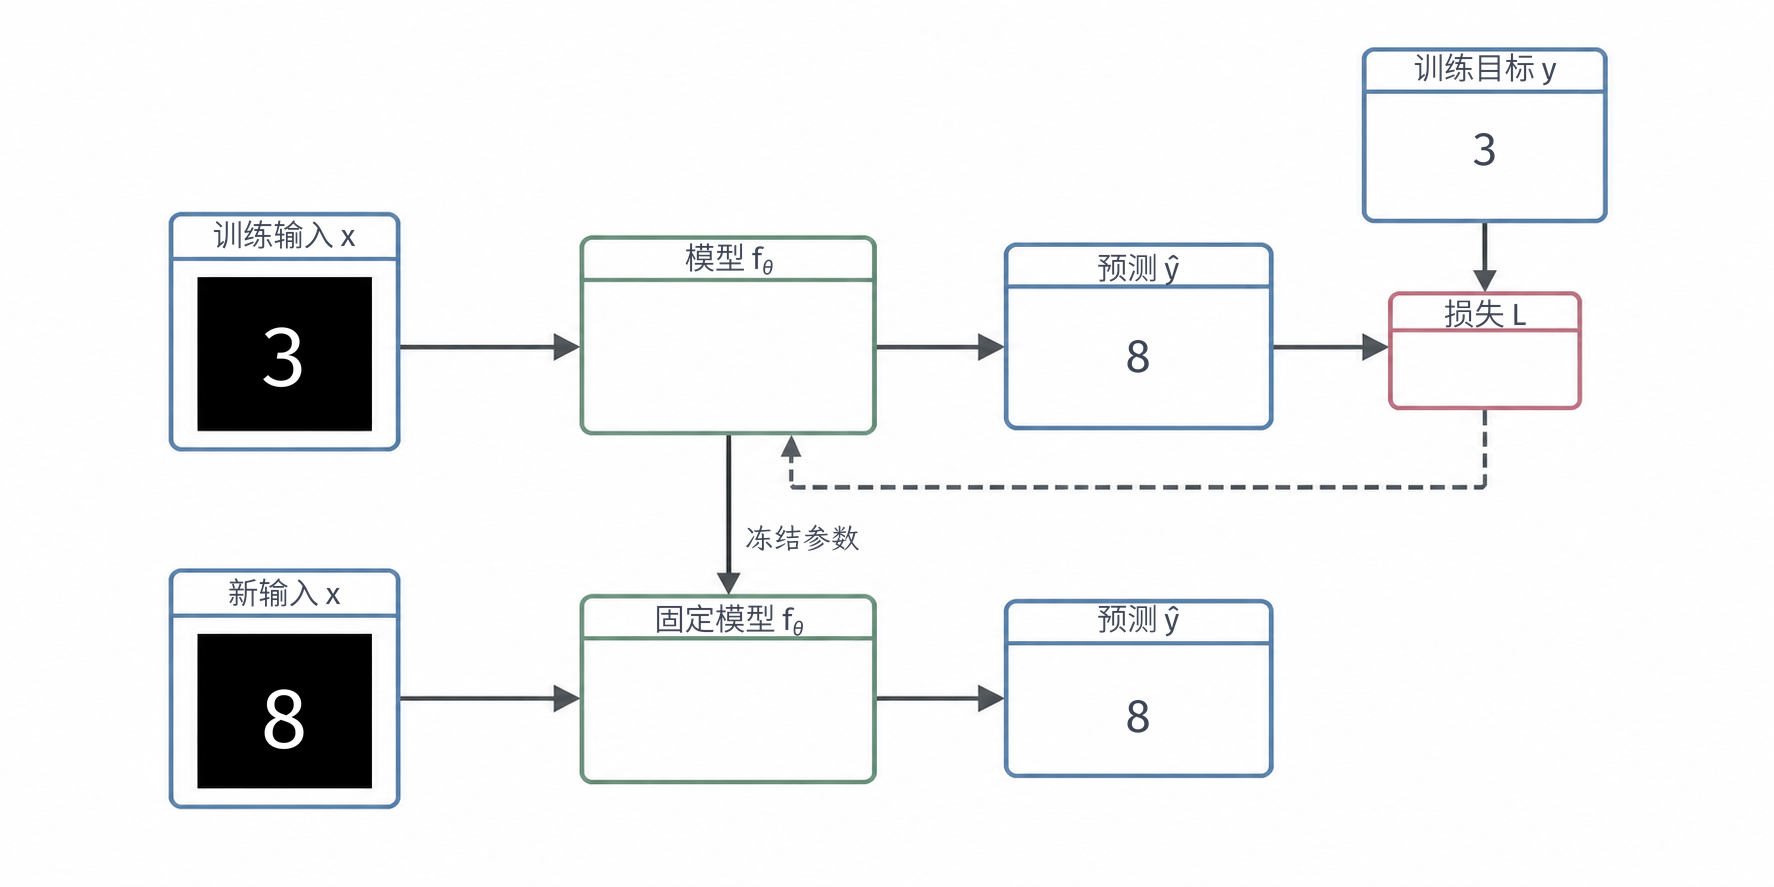
\includegraphics[width=164.600mm]{figures/03-foundations/01-basics/generated/supervised-learning/figure.png}
  \caption{监督学习中的训练与使用。训练时图像进入模型，目标标签单独进入损失比较，虚线反馈用于更新参数；使用时只提供新图像。训练行中，数字3被暂时预测为8，原标签3只进入比较；使用行没有提供目标。数字字形为教学构造，不是MNIST原始样本；模型框不指定网络架构。}
  \label{fig:supervised-mnist-process}
\end{figure*}
\FloatBarrier

可靠目标与样本覆盖共同限制监督学习。某类笔迹若从未进入训练集，或标签含有系统性错误，多训练几轮不能自动弥补；训练中的输入与目标关系能否延续到应用场景，也不能由数据集名称保证，而需在目标场景独立检验。标签规定了希望预测什么，有限标签却未必代表所有新情况。

\section{无监督学习}
\label{sec:unsupervised-learning}

现在考虑没有逐样本答案的一批新闻。我们仍可观察哪些词经常共现、哪些文档彼此相近，再用这些规律整理内容。这样从数据发现结构或分布，而不依赖逐样本目标答案的设定，称为\term{无监督学习}（unsupervised learning）。

要寻找的规律由用途决定。\term{聚类}（clustering）依照相似性形成群组，可用于探索购买行为；\term{降维}（dimensionality reduction）以较少变量保留重要变化或邻近关系，可服务于可视化、压缩和后续分析；\term{分布建模}（distribution modeling）描述观测出现的规律，可用于采样或识别不常见观测。没有标签并不妨碍设定这些目标，只是检查依据转向了数据及所作假设。

顾客聚类说明表示怎样影响发现的结构。只比较购买金额，群组可能主要区分消费水平；加入购买时间与商品种类，就可能反映不同购物习惯。算法可以反复调整分组，让组内样本在选定表示下更相似，但最终分组始终依赖所用特征与相似性标准。省去答案以后，学习目标和假设仍然存在。

一篇新闻可能同时涉及体育和经济，唯一群组会遗漏这种混合。潜在狄利克雷分配（latent Dirichlet allocation, LDA）因此用多个主题共同描述文档，各主题再由词语概率刻画。原始研究在16,000篇TREC AP新闻上学习100个主题，并观察各主题的高概率词\scite{blei2003}。文档没有预填主题标签；学习利用同一文档中的词语共现形成潜在主题，研究者随后根据代表词解释其含义。图~\ref{fig:unsupervised-topic-process}展示了整批文档提供统计规律、所得模型再描述新文档主题组成的过程。

\begin{figure*}[!htb]
  \centering
  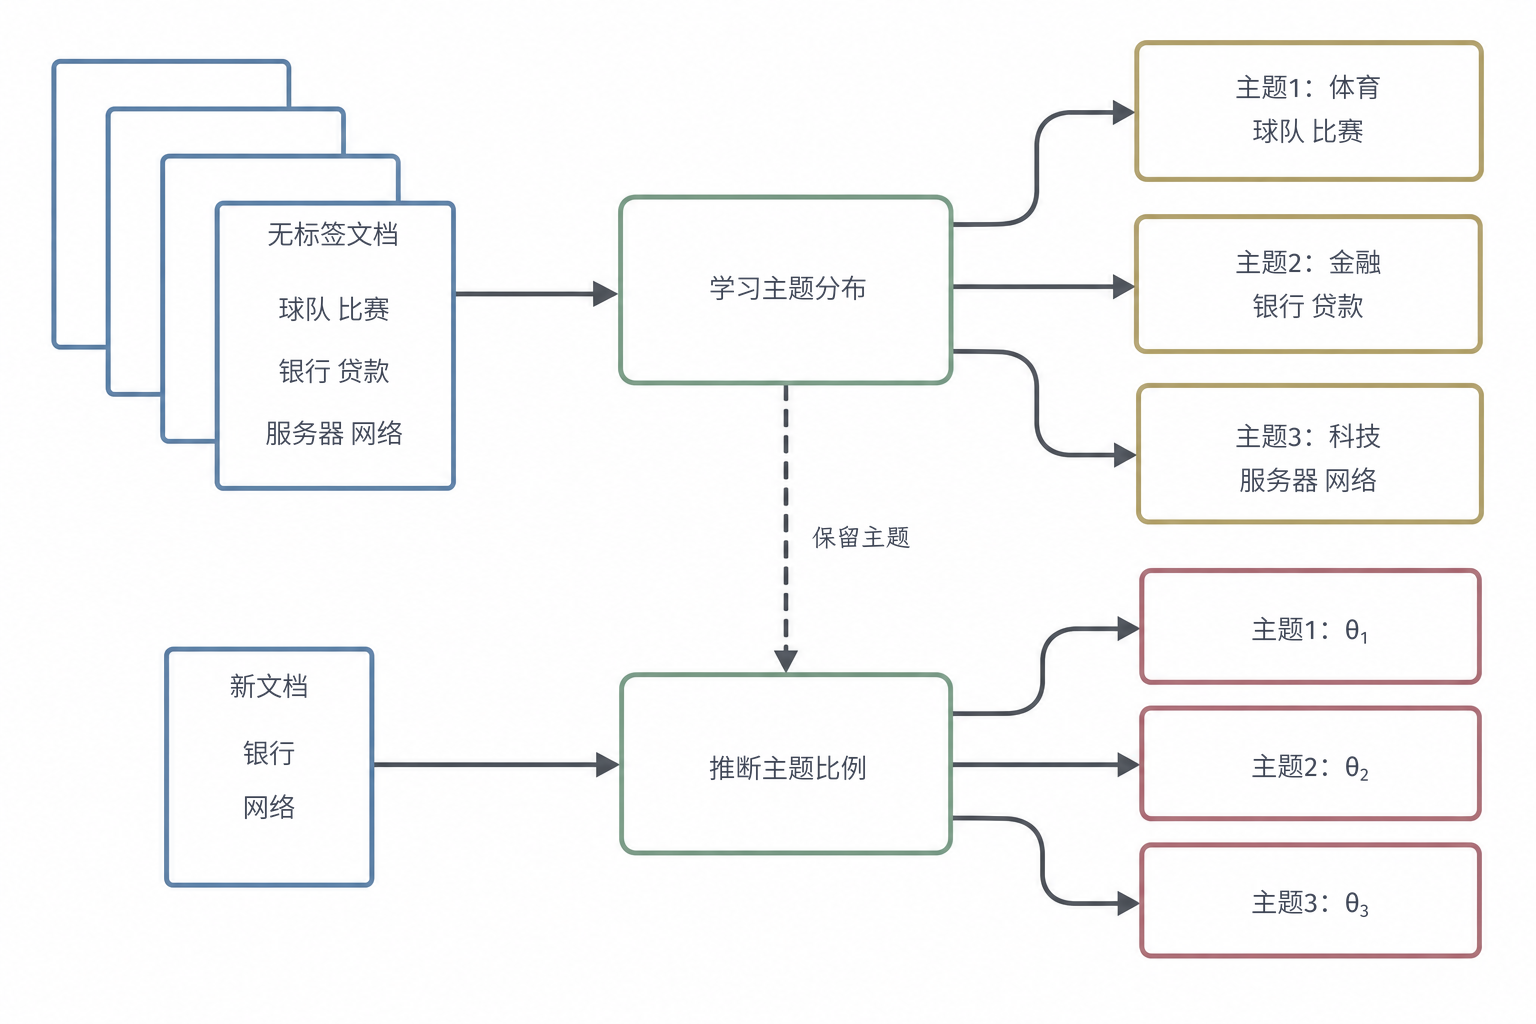
\includegraphics[width=164.600mm]{figures/03-foundations/01-basics/generated/unsupervised-topics/figure.png}
  \caption{无监督主题发现的过程示意。没有主题标签的新闻集合提供词语共现信息，学习过程形成
  若干潜在主题；同一篇文档可以由多个主题共同构成，主题名称是在结果解释阶段由人给出的。}
  \label{fig:unsupervised-topic-process}
\end{figure*}

若预先规定“体育”“财经”并提供类别示例，问题便是监督分类；主题发现则先学习共现模式，后由人解释和命名。事后把主题命名为“体育”，不会使这个名称成为训练时的标签。混合主题还允许同一新闻同时保留体育与经济成分。

发现的坐标和群组未必对应业务概念。把顾客的几十项特征压缩成两个坐标，可以画图观察邻近关系，但坐标轴未必具有“收入”或“年龄”的含义，分离的群组也未必是业务要区分的类型。计算出的结构与人赋予的解释需要分别检查。

新闻主题可以从三方面检查：代表词能否概括对应文档的内容，更换一批同来源新闻后各主题的高概率词是否大体保留，以及按主题整理是否减少人工查找相关文档的时间。它们分别提供解释、稳定性及实际用途的证据。图上群组清晰只呈现一种几何现象，还不足以证明结果有效。

\FloatBarrier
\section{强化学习}
\label{sec:reinforcement-learning}

下棋时，当前落子既改变棋盘，也改变之后的选择；机器人移动和车辆换道同样会改变后续处境。已有数据上的预测误差于是不能完整评价行动，我们还必须追踪它留下的后果。

利用行动后果的奖励学习决策，称为\term{强化学习}（reinforcement learning），通常以多步奖励构成的预期累计回报为目标。决策者称为\term{智能体}（agent），与之交互的外部世界称为\term{环境}（environment），环境给出的数值评价称为\term{奖励}（reward）。下棋程序作出落子，棋局与对手回应形成环境反馈；评价策略时还要考虑不同交互经历的平均结果。

智能体依据当前可用信息选择动作，所用规则称为\term{策略}（policy）。\term{状态}（state）描述环境处境，\term{观测}（observation）是智能体实际得到的信息。机器人摄像头只能看到某个方向，两者因而未必一致；必要时，策略要结合此前的观测和动作，不能把一帧画面直接当作完整状态。

建立基准时，我们先固定任务与单个智能体，并采用Markov状态。按第一卷有限时域口径，马尔可夫决策过程（Markov decision process, MDP）规定状态集、可选动作、初始状态分布、受控转移、阶段及终点奖励和时域。给定当前状态与动作后，下一状态和奖励的分布不再依赖更早历史，这就是Markov条件。状态是否可见、转移是否已知、经验来自在线交互还是固定记录，则属于学习者的信息及访问条件，会改变方法和评价协议，不属于MDP元组本身。

标签直接提供希望预测的对象，奖励通常只评价已采取动作的结果，并不列出正确动作。反馈还可能延迟：围棋的胜负要到终局才能确定，当前吃子较多并不保证最终获胜。强化学习因而需要关联当前选择与后续结果，不能把即时得分直接等同于长期目标。

策略、轨迹、折扣及长期平均回报已在\BookSectionRef{sec:policy-trajectory-return}{第一卷“策略的价值与优化”章的“轨迹与回报”一节}定义。辨认范式时，我们检查策略与环境怎样产生轨迹，训练怎样使用过程或终点奖励，而不只看模型是否连续输出动作。\term{折扣因子}（discount factor）、平均方式和风险准则还会改变长期表现的含义，需要一并限定\scite{sutton2018}。

在线交互中，当前策略产生观测、动作和奖励记录，算法用记录评价长期后果并调整策略；新的策略又会改变下一轮经历。只重复已知有效的动作，可能错失更优选择；不断尝试未知动作，则可能牺牲已有收益。探索与利用的权衡因此同时涉及获取信息和取得回报\scite{sutton2018}。

这些记录可以按不同方式进入策略改进。价值方法先估计状态或动作的长期后果，再据此选择；直接策略优化使用回报信号调整策略；\term{行动者—评论家}（actor--critic）同时维护策略和价值估计，让后者评价前者的更新。它们说明价值估计与策略更新怎样配合，具体算法由第四卷展开。

若能预测动作将怎样改变状态或观测及奖励，就可以在行动前比较后果。描述这类变化的\term{环境模型}（environment model）可以已知，也可以从数据学习，之后用于规划。模型提供了比较路径，评价仍需关联即时反馈与长期结果。

2015年的深度Q网络（deep Q-network, DQN）研究在49款Atari游戏上采用相同基本算法和模型设定，利用游戏画面及分数学会控制\scite{mnih2015}。智能体看画面、选按键，环境返回新画面与分数，再形成下一批经验。DQN采用价值方法，估计按键可能带来的累计回报，而非只预测即时加分；游戏分数也没有直接告诉它应按哪个键。图~\ref{fig:reinforcement-atari-process}借机器人探索展示同一分工：动作改变处境，后续观测与奖励进入学习。

\begin{figure*}[t]
  \centering
  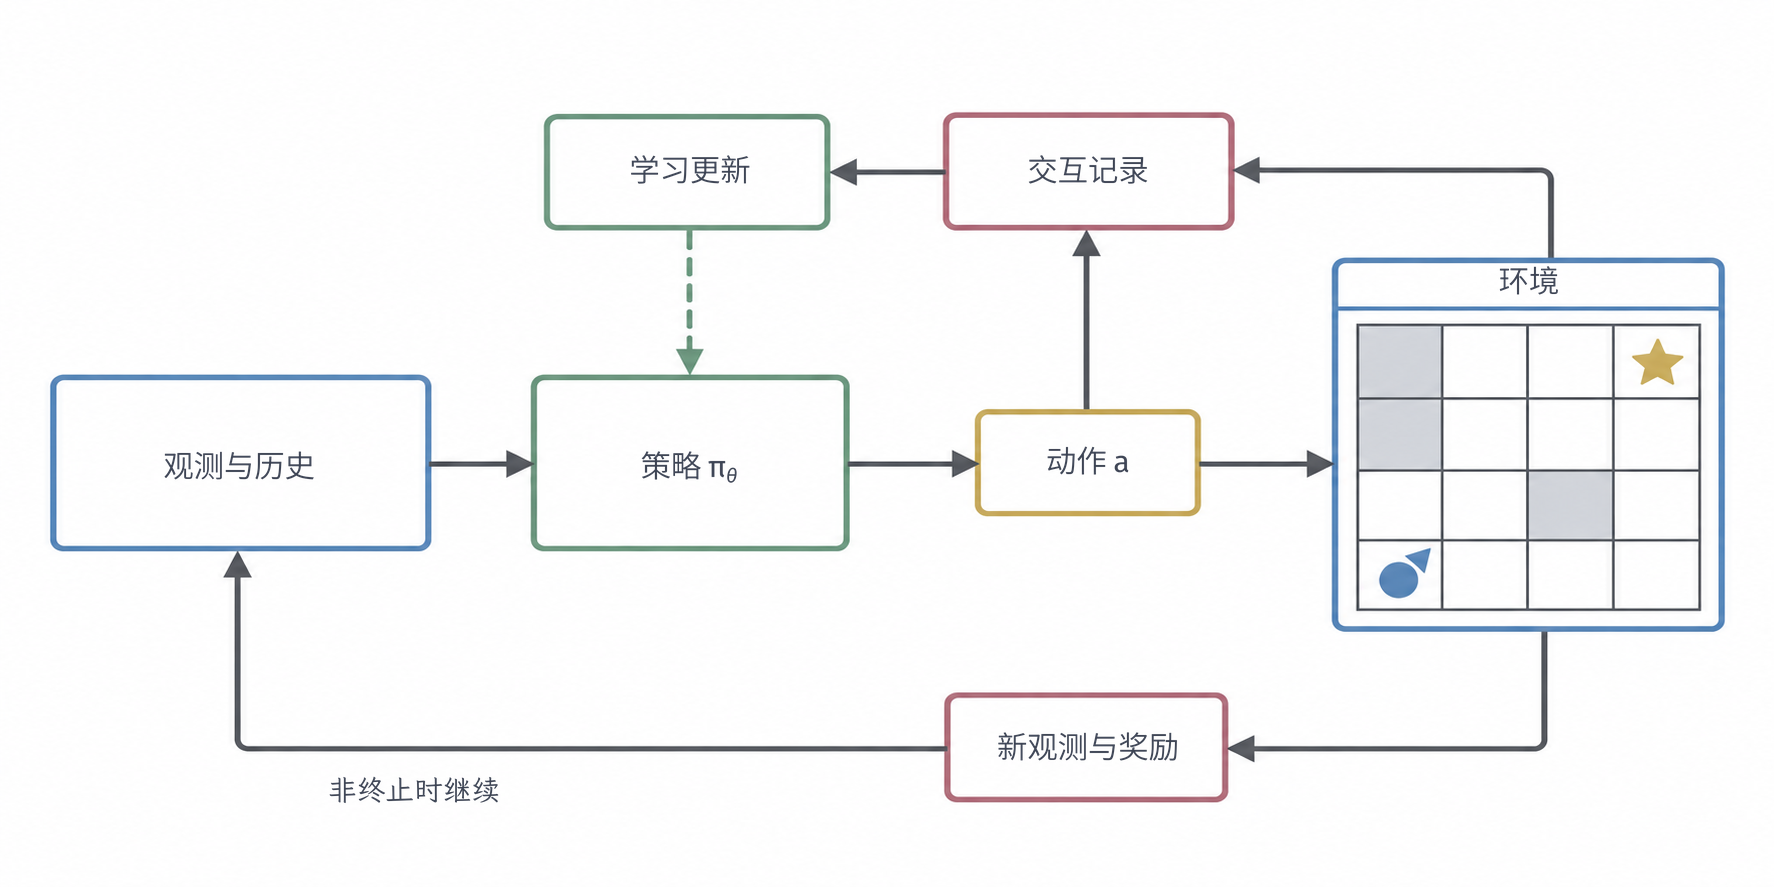
\includegraphics[width=164.600mm]{figures/03-foundations/01-basics/generated/reinforcement-loop/figure.png}
  \caption{机器人探索中的强化学习交互。策略依据观测与历史选择动作，环境返回新观测与奖励；动作和环境反馈共同形成交互记录，学习过程据此更新策略，非终止时继续交互。格图中的机器人、障碍与目标仅为概念场景，不表示测量结果、精确状态转移或回合终止。奖励不是正确动作标签。}
  \label{fig:reinforcement-atari-process}
\end{figure*}

围棋中，棋盘对应状态，落子对应动作，终局胜负提供关键反馈。自我对弈可以继续产生棋局，让后续胜负用于学习不同局面的行动。第~\ref{sec:combining-learning-paradigms}节以AlphaGo说明这类经验怎样与人类棋谱配合。

机器人可从摄像头、关节位置及力传感器取得观测，再选择移动关节、改变抓取姿态或行走方向。奖励可以评价抓取是否稳固、目标是否到达，以及动作是否平稳。不过，真实失败可能损坏设备，不能像游戏一样简单重开，取得经验本身就带有成本。

跟车、换道和路径规划也可写成序贯决策：车辆选择动作后，位置、速度及其他车辆的回应共同形成新状态，评价兼顾安全、效率与舒适。整个自动驾驶系统却包含不同学习问题，感知可利用监督或自监督反馈，决策需追踪动作后果。推荐、调度和能源管理也可能需要这种建模，是否采用强化学习要依据反馈与长期目标判断。

新闻推荐可以先采用简化设定：只检查展示后是否点击，不建模本次推荐怎样改变后续兴趣。但系统仍只能观察已选新闻的反馈，无法同时知道其他选择的结果。反复选择并积累这种奖励，构成\term{多臂老虎机问题}（multi-armed bandit）；选择前若还可见用户特征和候选新闻等信息，则构成\term{上下文老虎机问题}（contextual bandit）。Li等人的推荐研究采用后一设定\scite{li2010bandit}。

老虎机设定不让当前动作通过改变环境状态影响后续奖励，但当前反馈会增加信息，影响之后的选择，仍存在探索与利用。若推荐对未来行为的影响也进入目标，就要扩大为序贯决策模型。因此，应用名称不能决定设定，关键是哪些行动后果被纳入评价。

无法承担在线试错时，可以先用模拟器学习，或以专家示范建立初始行为。\term{离线强化学习}（offline reinforcement learning）则使用已经收集的交互记录，学习时不再额外与环境交互\scite{levine2020offline}。这些途径减少真实试错，却各有经验限制：模拟器可能失配，示范可能错误或覆盖不足，历史记录也可能缺少将来重要的状态和动作。所得策略仍需检验，再逐步投入使用。

经验充分也不保证奖励完整表达任务。只奖励机器人迅速搬运，可能忽略物体受损；我们需要把损坏纳入评价，并为不可接受的行为加入约束。难以直接数值化的要求，可通过人对结果的偏好学习评价信号，也可由规则或验证器检查过程与最终结果。第~\ref{sec:combining-learning-paradigms}节会介绍偏好与强化学习的组合。无论信号怎样构造，成功仍应依据实际任务要求检查，奖励提高不能替代这一判断。

示范还能直接提供动作依据：专家展示某种处境下的行动，学习者据此学习行为，称为\term{模仿学习}（imitation learning）。其中\term{行为克隆}（behavior cloning）把专家观测与动作配成输入和目标，采用监督学习。

但学习者一旦走偏，就可能遇到示范中没有的处境，随后错误继续累积。DAgger让学习者实际行动，再请专家为遇到的状态提供动作，补充原示范的覆盖\scite{ross2011}。模仿与强化学习均可生成连续行动，区别在于训练主要使用动作示范还是结果奖励，不能只看使用时的行为形式。

示范也可用于推断专家为何选择这些动作。\term{逆强化学习}（inverse reinforcement learning）寻找能够解释示范的奖励函数，再用它学习策略\scite{ng2000irl}。路线可以反映对路程、障碍及安全距离的取舍，但同一行为往往符合多种奖励，有限示范一般不能唯一还原真实目标。推得奖励以后，还需检查它引导的行为。

上述基准固定任务和决策者，以期望回报比较策略。应用还可能要求跨任务复用经验、与其他会学习的参与者协作或博弈，以及控制严重损失、扰动和不安全行为。这分别改变任务、参与者和行为要求，平均训练奖励不能同时证明它们满足。可靠性评价必须限定运行范围、失败指标与证据，有限测试不能外推为任意环境保证。

\BookPartRef{part:reinforcement-learning}{第四卷“范式”的“强化学习”部分}将沿这些问题展开：环境模型已知或未知时如何规划与学习，观测和经验受限时怎样决策，奖励难以获取或表达不准时怎样形成反馈，以及任务、参与者、风险和安全要求变化时怎样评价策略。

\section{知识的获取}
\label{sec:efficient-knowledge-use-overview}

收集照片通常比确认物种容易，可靠任务标签因而可能成为学习的限制。预算有限时，我们要考虑让已有标签发挥更大作用、利用其余原始数据，或选择更值得新增标注的样本。这里关注的是训练依据怎样取得和使用。

训练依据不限于类别标签。我们把可指导训练的答案、样本关系、约束与目标统称为训练知识。人工、规则、模型和数据产生的内容在核验前都是候选知识；数量、置信度或训练损失均不能单独证明质量。知识不足也可能是覆盖不全、粒度失配、内容错误或过时，需要分别处理。

本节所谓高效，是在达到同一目标评价要求时减少人工任务标签，或在相同标注预算下相对于既定基线改善独立评价结果。它不承诺计算更少。比较时，应分别报告任务收益及人工、模型调用、计算和维护成本，而不能用候选标签或样本的新增数量代替收益。

我们先按半监督、自监督、弱监督、对比及主动学习辨认资源和训练信号。\BookPartRef{part:efficient-knowledge-use}{第四卷“范式”的“知识的获取”部分}再按来源与处理职责组织：人工、规则、模型和数据提供候选依据，之后进行融合、评估与修正。两种组织并非一一对应。主动学习选择向人工询问的样本，标注函数使用规则，伪标签、教师输出和生成材料来自模型，自监督、对比及分组从数据内容或关系构造目标；半监督和弱监督可以合用多个来源。

\subsection{半监督学习}
\label{sec:semi-supervised-learning}

商品类别已确定，但只有少量图片完成标注时，标签可以规定类别含义，其余图片可能补充光照、角度与背景的变化。\term{半监督学习}（semi-supervised learning）让有标签与无标签数据共同服务于目标任务，利用后者提供的输入规律扩展学习。

无标签图片如何进入训练？\term{自训练}（self-training）先以已有标签训练模型，再预测其余样本；采纳为临时目标的预测称为\term{伪标签}（pseudo-label）。原标签与选中伪标签一起参与后续学习，之后还可重新生成。预测提供了使用额外数据的途径，却没有因此成为真实答案。

筛选常依据\term{置信度}（confidence），即模型对当前预测的确定程度；分类时常以预测类别的概率作为置信度分数。但自信也可能伴随错误，反复学习错误伪标签会强化原误判。因此，筛选之外还需控制伪标签的权重或影响，不能将高置信度直接当作可靠性证据。

还可以不先决定类别，而是约束同一对象的预测。轻微改变亮度通常应保留动物类别，要求变换前后预测稳定便是\term{一致性约束}（consistency regularization）。同一原图产生的不同\term{视图}即使无标签，也能提供预测分歧作为调整依据。前提是变换保留任务含义：裁剪若删除动物，要求类别不变反而会误导模型。

样本之间的相似性提供另一条途径。\term{基于图的方法}（graph-based methods）将样本作为节点、相似关系作为边，再让少量标签影响邻近无标签节点。经典图半监督方法以两类样本共同构图，要求相邻预测接近\scite{zhu2003}；聚类思路则假设密集群组往往对应同类。两者都需要任务相关的相似性，背景颜色相近并不保证类别相同。

FixMatch将伪标签与一致性合用：先预测弱变换的无标签图片，最大类别概率达到预设阈值时采用其类别，再要求同图强变换后的预测一致\scite{sohn2020}。真实标签约束类别含义，这两项要求把训练延伸到没有提供答案的图片。

CIFAR-10有十类物体，相关实验只揭示少量训练图的类别，其余训练图参与上述过程。这里的无标签指答案被隐藏，训练不得读取原本保存的真实类别。图~\ref{fig:semi-supervised-image-process}说明两路数据怎样共同用于分类。

\begin{figure*}[!htb]
  \centering
  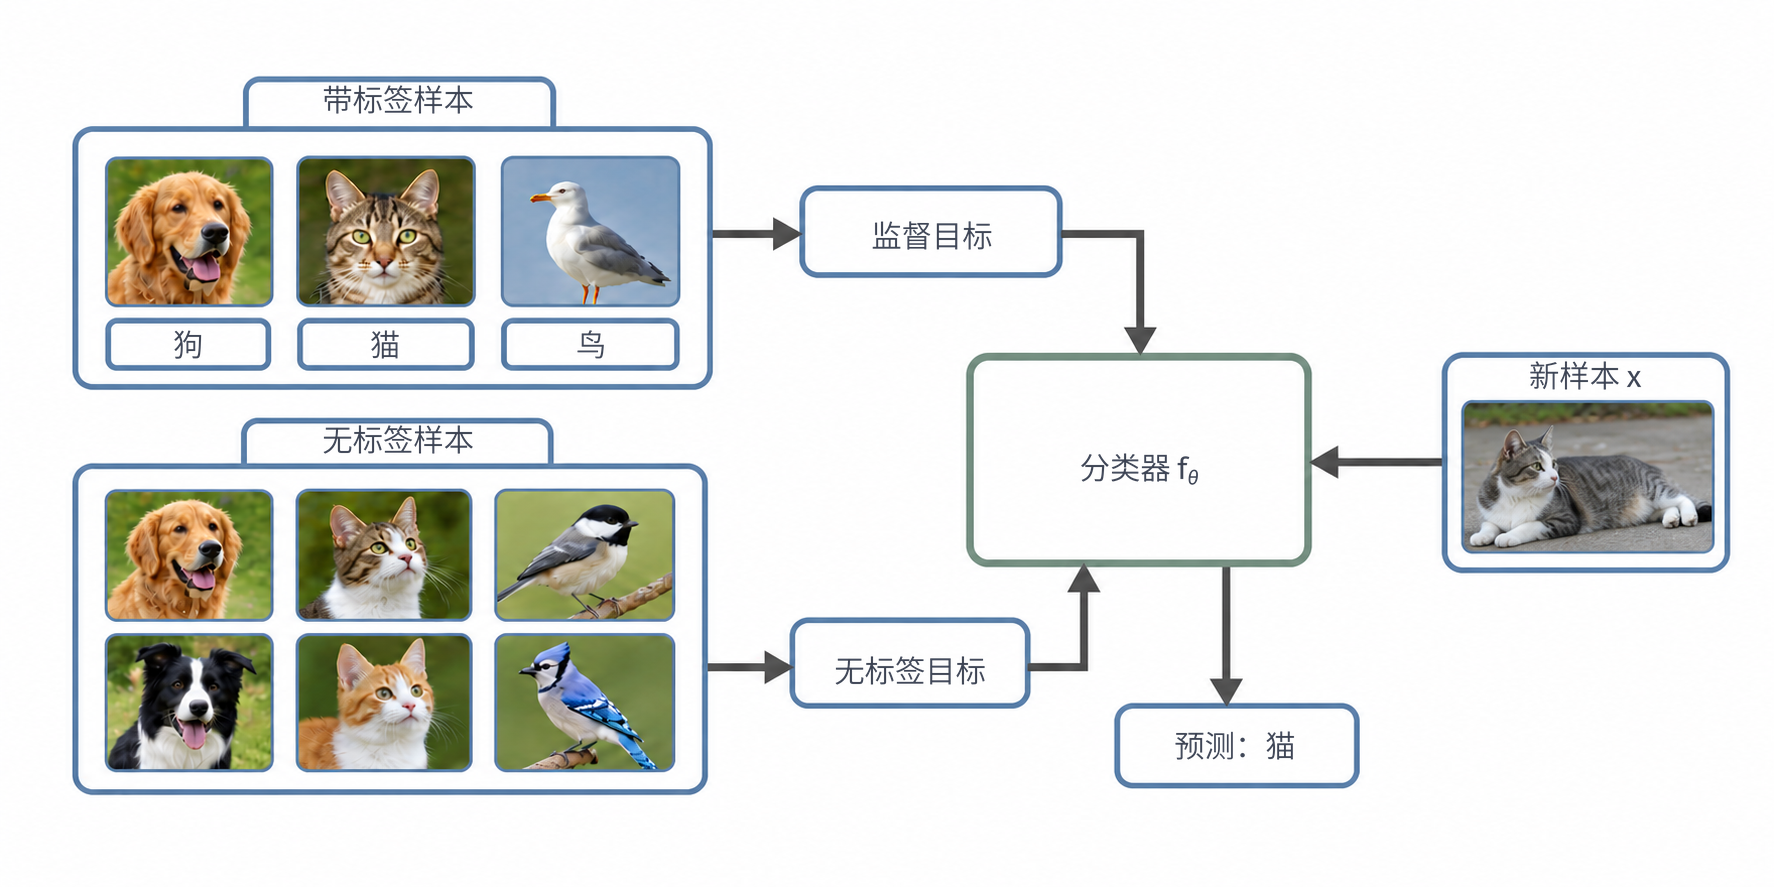
\includegraphics[width=164.600mm]{figures/03-foundations/01-basics/generated/semi-supervised-learning/figure.png}
  \caption{半监督学习的过程示意。少量带类别标签的图片规定目标，大量无标签图片提供额外结构信息，两路经验共同用于形成分类能力，汇入同一分类器。模型框不指定网络结构；动物图片为教学构造。无标签图片的隐藏真值不能作为训练答案使用。}
  \label{fig:semi-supervised-image-process}
\end{figure*}
\FloatBarrier

这个设定还要求额外图片与十类识别任务相关。若加入类别范围之外的图片，模型可能仍自信地赋予已知类别，再将它作为伪标签学习。额外数据的适用范围因而需要检查，数量增加本身并不保证帮助。

预测范围也需明确。若学习一条处理未来新输入的规则，称为\term{归纳学习}（inductive learning）；若待预测图片已给定，学习利用其结构为这批特定输入补全答案，称为\term{直推学习}（transductive learning），也称转导学习。直推支持向量机采用了预先给定待分类样本的设定\scite{joachims1999transductive}。

归纳与直推限定输入可见性及评价范围，半监督则限定标签资源，两者是不同维度。半监督可以使用任一种预测设定。直推允许查看待预测输入，却仍应隐藏它们的答案；这批输入上的评价也不能替代未来新样本的表现。

半监督仍用已有类别标签规定任务。若这些标签尚不存在，我们可以从原始数据构造别的有答案问题，先学习日后可能复用的规律。

\subsection{自监督学习}
\label{sec:self-supervised-learning}

完整文本没有情感标签，却保留着每个词。暂时隐藏一部分内容，就能以可见上下文为问题、原内容为答案，构造无需另行标注的训练示例。这为标签稀缺提供了另一种训练依据。

从数据内容或关系构造目标，称为\term{自监督学习}（self-supervised learning）。遮挡恢复、后续内容预测和不同视图匹配都可采用这种方式。“自”限定目标来源，遮什么、比什么仍需设计。我们希望补词促成语法与语义学习、图像恢复促成纹理和物体关系学习，但究竟获得哪些能力还需用实际任务检验。

BERT的掩码预测给出具体过程\scite{devlin2019}。文本先分成\term{词元}（token），它可以是字、词或词的一部分；训练随机选择部分词元，将其中多数换成掩码，再用左右上下文预测原词元。原文同时提供输入与答案。例如教学句子“猫在垫子上”隐藏“垫子”后，剩余内容进入模型，原词元单独用于比较。图~\ref{fig:self-supervised-masked-process}展示了两路信息，模型预测时不能读到保留答案。

\begin{figure*}[!tbp]
  \centering
  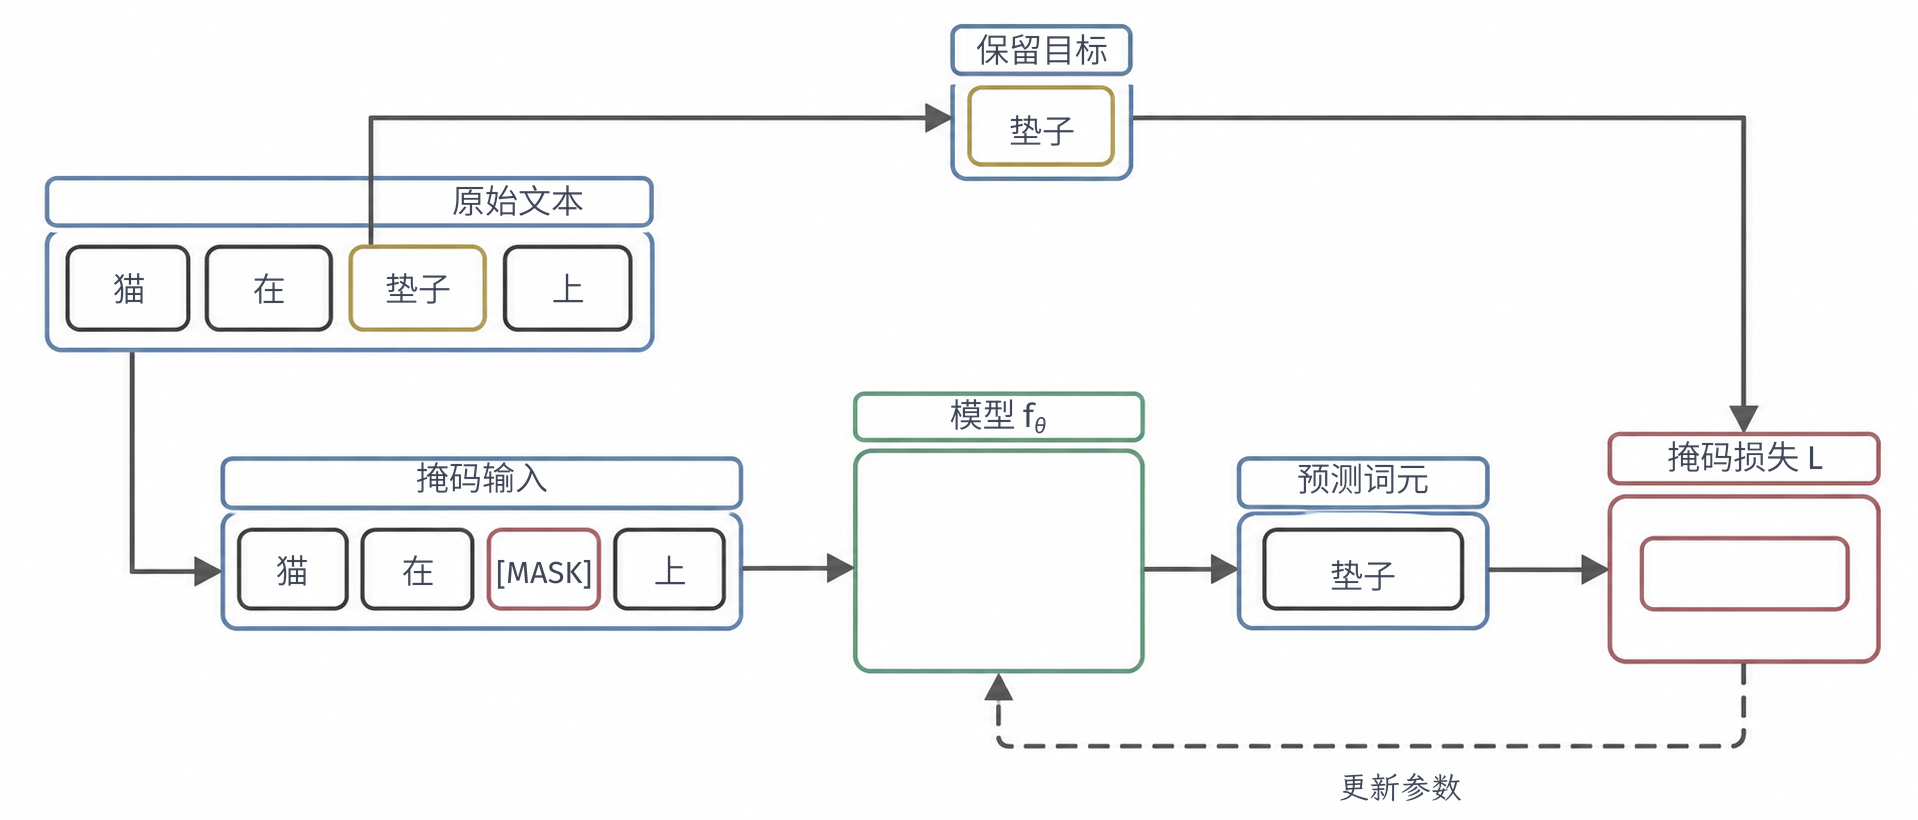
\includegraphics[width=164.600mm]{figures/03-foundations/01-basics/generated/masked-self-supervision/figure.png}
  \caption{掩码预测以“猫在垫子上”为教学例子。输入将“垫子”替换为[MASK]，原词单独保留为比较目标；模型只能读可见上下文，不能读被保留的答案。可见词元共同进入模型，灰色虚线将损失反馈到参数；模型框不指定网络结构。}
  \label{fig:self-supervised-masked-process}
\end{figure*}
\FloatBarrier

配对构造完毕，就可比较预测与答案并调整参数。下一词元预测只以目标之前的文本为输入，以紧随其后的原词元为答案，也能批量生成示例。辨认自监督时应追溯目标的构造：掩码任务恢复原文，情感分类则预测另行规定的评价类别。是否人工手填标签并不足以区分二者。

同一批新闻还可用于前述主题发现。主题模型从共现学习潜在结构，掩码任务则把数据转换成显式输入和恢复目标，逐次比较预测与答案。二者都利用缺少人工任务标签的数据，也都包含目标和人为假设；差别并非是否存在目标函数。

广义无监督学习可包含自监督，因为它不依赖额外人工任务标签。本书为说明信号怎样构造，将自监督单列讨论；这是一种内容组织方式，而非要求分类互斥。

自监督目标可直接用于文本生成，也可先学习表示，再服务分类或问答。先积累可复用知识的阶段称为\term{预训练}（pre-training），后续具体用途称为\term{下游任务}（downstream task）。例如，先学习文本与上下文关系，再用少量情感标签学习评论类别；两个阶段利用的目标来源不同。

预训练所得规律还不能自动规定下游类别，最终任务可能需要标签或其他说明。构造目标也可能让模型走捷径：若局部词语搭配足以恢复遮挡，完成该目标未必要求理解整段文字。因此，是否帮助下游任务，要以实际评价为依据。

\subsection{弱监督学习}
\label{sec:weakly-supervised-learning}

还可利用成本较低、质量不完善的现有标注。汽车定位需要位置答案，但现有数据可能只注明“图中有汽车”，甚至网页标签与内容不符。\term{弱监督学习}（weakly supervised learning）研究怎样利用不完整、不精确或不可靠的监督，让学习不必等到所有标注达到理想标准才开始。

一种常用划分把部分样本缺少标签称为\emph{监督不完整}（incomplete supervision），把整图类别不能提供位置等所需信息称为\emph{监督不精确}（inexact supervision），把标签与内容不符称为\emph{监督不准确}（inaccurate supervision）\scite{zhou2018}。第~\ref{sec:semi-supervised-learning}节的半监督学习主要处理第一种，属于广义弱监督范围。本节转向粗粒度、错误标签和规则监督。

领域经验也可先转成批量规则。Snorkel允许专家编写\term{标注函数}（labeling function），依据关键词、模式或外部知识作判断，并在依据不足时弃权。例如，“含链接”提示垃圾评论，也可能误伤正常分享。系统综合一致、冲突与弃权的规则输出，估计类别概率，再以概率标签训练最终模型\scite{ratner2017}。图~\ref{fig:weak-supervision-process}中的汇合，表示从多条候选判断形成训练监督，而非直接确认真值。

规则还可来自事实关联、类别约束或结构要求，产生标签、候选范围及关系判断。未触发只表示没有给出判断，不能自动记为负例。使用时应记录规则的形成依据、适用对象和冲突处理方式，才知道候选信号代表什么。

批量规则减少逐条标注，也会传播自身局限。多条规则都依据链接，即使一致也可能共同误判正常分享；粗标签则可能缺少任务需要的位置细节。最终模型仍需独立可靠标签评价，符合规则不能证明已学会目标能力。

\begin{figure*}[htbp]
  \centering
  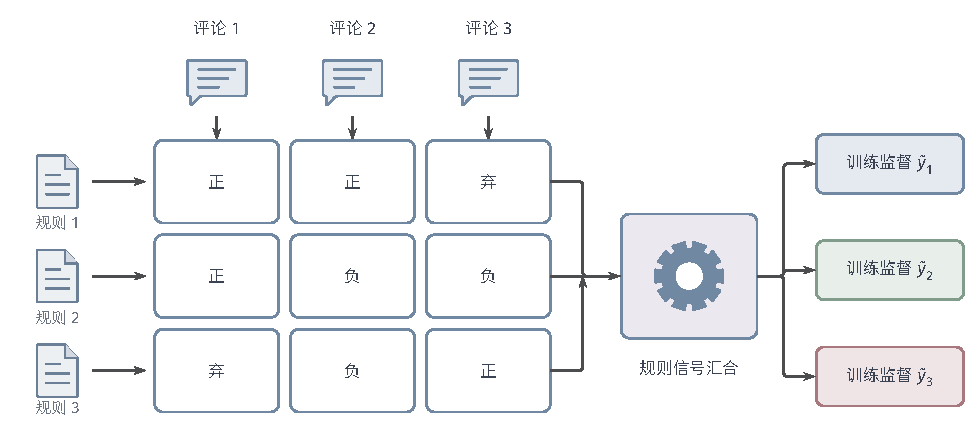
\includegraphics[width=164.600mm]{figures/03-foundations/01-basics/tikz/weak-supervision/figure.pdf}
  \caption{三条规则在三个未标注评论上的教学投票。正、负、弃分别表示两种倾向与弃票；同一列可能存在冲突。综合规则信号形成训练监督$\tilde y_i$，图中不规定合并算法，也不把某条规则输出等同于真实标签；评价仍使用独立可靠标签。}
  \label{fig:weak-supervision-process}
\end{figure*}
\FloatBarrier

从整图标签学习位置，需要把粗监督与区域预测联系起来。我们可把图像视为多个候选区域：整图有汽车，意味着至少一个区域包含汽车，而非每个区域都是汽车。这是\term{多示例学习}（multiple-instance learning）的典型设定，监督约束对象组而未逐一给出答案。若把整图标签复制到每个区域，背景就会被错误标为汽车。

对\emph{带噪声标签}（noisy labels），可以识别可疑样本并减弱其影响，也可建立标签出错的模型，例如用少量核验样本估计可靠性，再调整训练。但难学不等于错标，少见而正确的情形同样会令模型犯错。处理弱监督要利用已知不确定性，避免无条件把现有记录当作真值。

多来源规则通常先经过可靠性估计和综合，再与原始样本一起训练最终模型。综合时不能把近似规则当作独立证据：仅关键词略有差异的两条规则可能重复同一线索。来源的准确性、覆盖及依赖关系需要进入处理，并允许保留不确定结果。

规则之后继续训练，是希望模型从原内容学习更可推广的关系，处理规则未覆盖的输入。但规则中的系统性错误也可能被继承，所以这一步是否成功，要由独立样本上的可靠评价决定。

\subsection{对比学习}
\label{sec:contrastive-learning}

已知对应关系也可直接指导表示。一张照片改变颜色或取景后，两个视图同出一图这一关系仍可已知，无需先有类别标签。\term{对比学习}（contrastive learning）利用匹配与不匹配关系构造目标：使用相似度或匹配得分时，提高匹配对、降低对照对的数值；使用距离时，则缩短匹配距离、增大对照距离。希望匹配的对象构成\term{正样本对}（positive pair），不匹配对照构成\term{负样本对}（negative pair）。正负限定的是关系，不能与二分类类别混淆；距离或相似度的选取还需符合表示及下游用途。

SimCLR先用没有提供类别标签的图片学习表示，再检验这些表示是否帮助分类。原研究在ImageNet等数据上开展这一过程，之后用标签训练分类器或调整模型\scite{chen2020}。类别标签进入评价或后续训练，并未进入前一阶段的匹配构造。

具体目标是找出同一原图的另一个视图。每批原图各经两组随机裁剪、颜色变化等变换，再由共享模型形成表示；同源视图互相匹配，其余原图的视图提供对照。只要求同源接近，会允许所有图都映为同一点；加入对照，才同时要求保留变换下的联系及不同图片之间的差别。

图~\ref{fig:contrastive-learning-process}用两个同源视图和另一幅猫图作对照。模型在此不知道“鸟”“猫”类别，信号来自视图的原图来源，所以属于自监督。反复比较可能促成变换下稳定的特征，后续再检验分类用途。图中位置只表示训练所要求的关系，并非实验测得的表示分布。

\begin{figure*}[htbp]
  \centering
  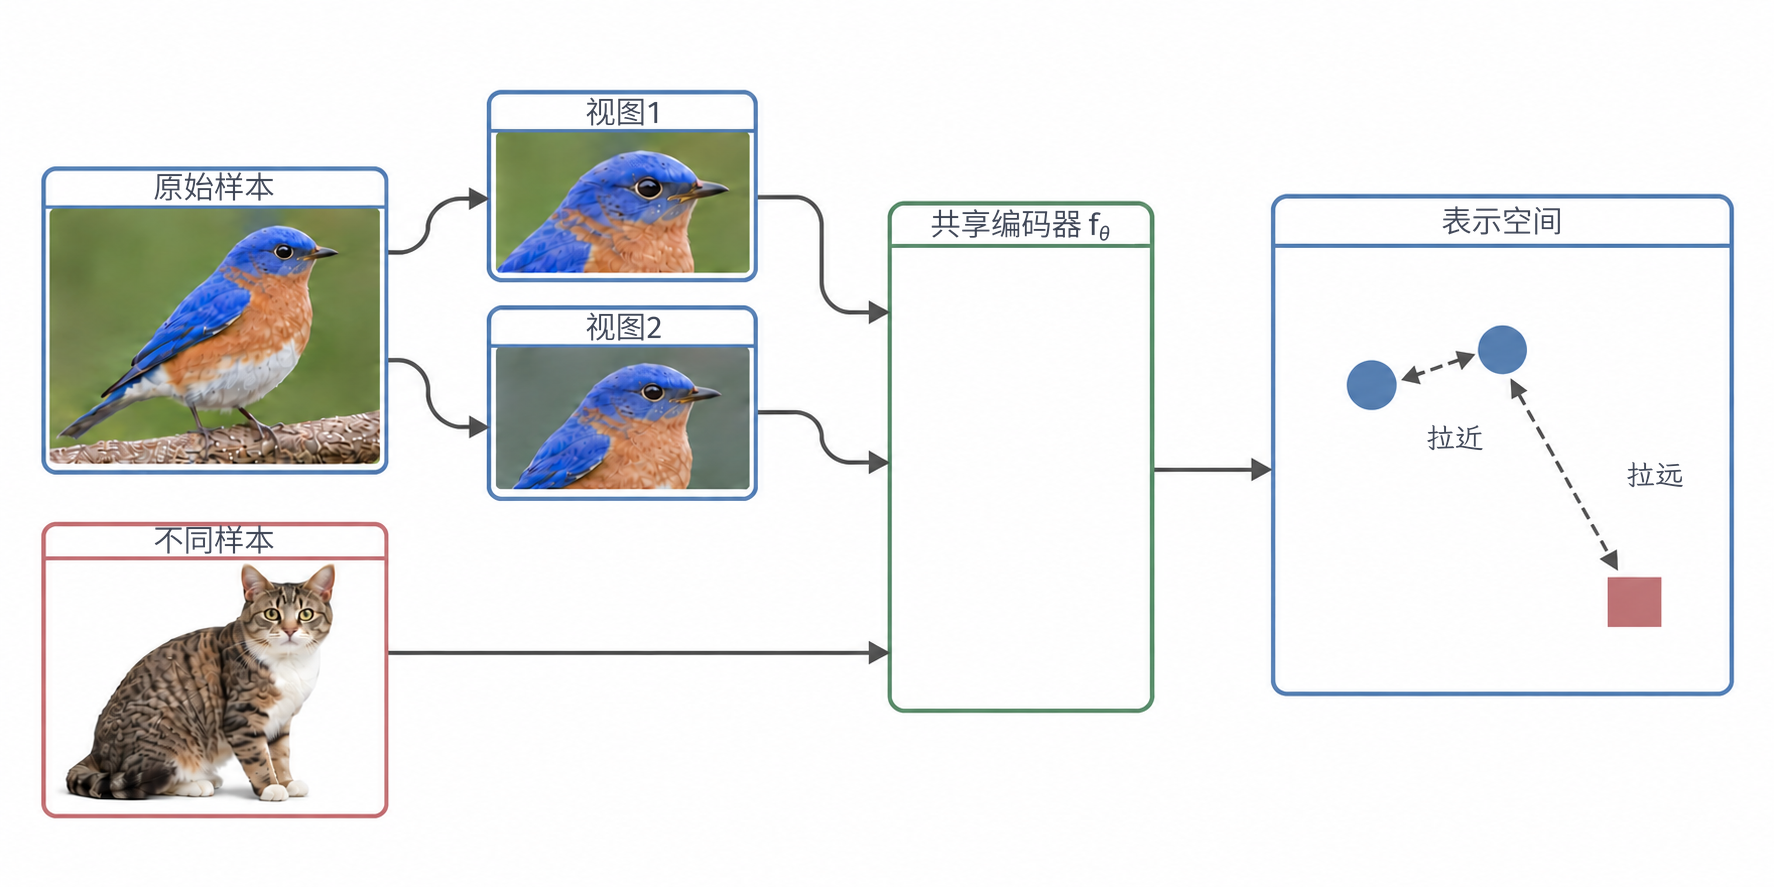
\includegraphics[width=164.600mm]{figures/03-foundations/01-basics/generated/contrastive-learning/figure.png}
  \caption{自监督对比学习的教学示意。同一幅鸟的原图分别经裁剪与颜色变化形成两个视图；它们与另一幅猫图的视图经共享参数的编码器得到表示。两个蓝色点表示同源视图的表示，红色点表示其他原图的对照；箭头只示意同源拉近与对照相对分离的训练目标。动物图元和表示位置均为教学构造，不是实测影像或表示分布。}
  \label{fig:contrastive-learning-process}
\end{figure*}
\FloatBarrier

匹配也可以由类别标签定义，形成监督式对比学习\scite{khosla2020}；还可匹配图像和描述它的文字。因此，对比限定目标的构造，自监督限定信号来源。SimCLR兼具两者，掩码预测则使用自监督来源而未采用对比目标。

这些关系还需服从任务含义。裁剪若改变内容，同源视图未必仍适合匹配；不同原图若拍摄语义相近对象，把它们一律作为负对照可能妨碍后续分类。采用对比目标前，需要检查哪些差别应保留、哪些变化应忽略。

\subsection{主动学习}
\label{sec:active-learning}

若能补充标签但预算有限，我们还需决定为哪些样本补充标签。\term{主动学习}（active learning）根据当前知识选择样本，再请人或其他可靠来源提供答案，希望有限查询补足覆盖或纠正错误。这里的选择对象是新增标签的获取位置。

池式设定需要未标注样本池、当前模型、可回答查询的来源及预算。相关输入尚未收集或回答来源不可靠时，主动选样本身不能补齐缺失信息。因此，查询策略的作用以这些资源可用为前提。

Gal等人的MNIST研究从20张类别均衡的标注图开始，每轮查询10张，再学习并与随机选样等准则比较\scite{gal2017}。基准中的查询只是揭示已保存但对模型隐藏的标签，未必由现场标注者实时作答；应用中则可由医生、工程师或普通标注者提供。图~\ref{fig:active-learning-loop}展示新标签进入模型之后，下一轮选择随知识变化的循环。

\begin{figure*}[htbp]
  \centering
  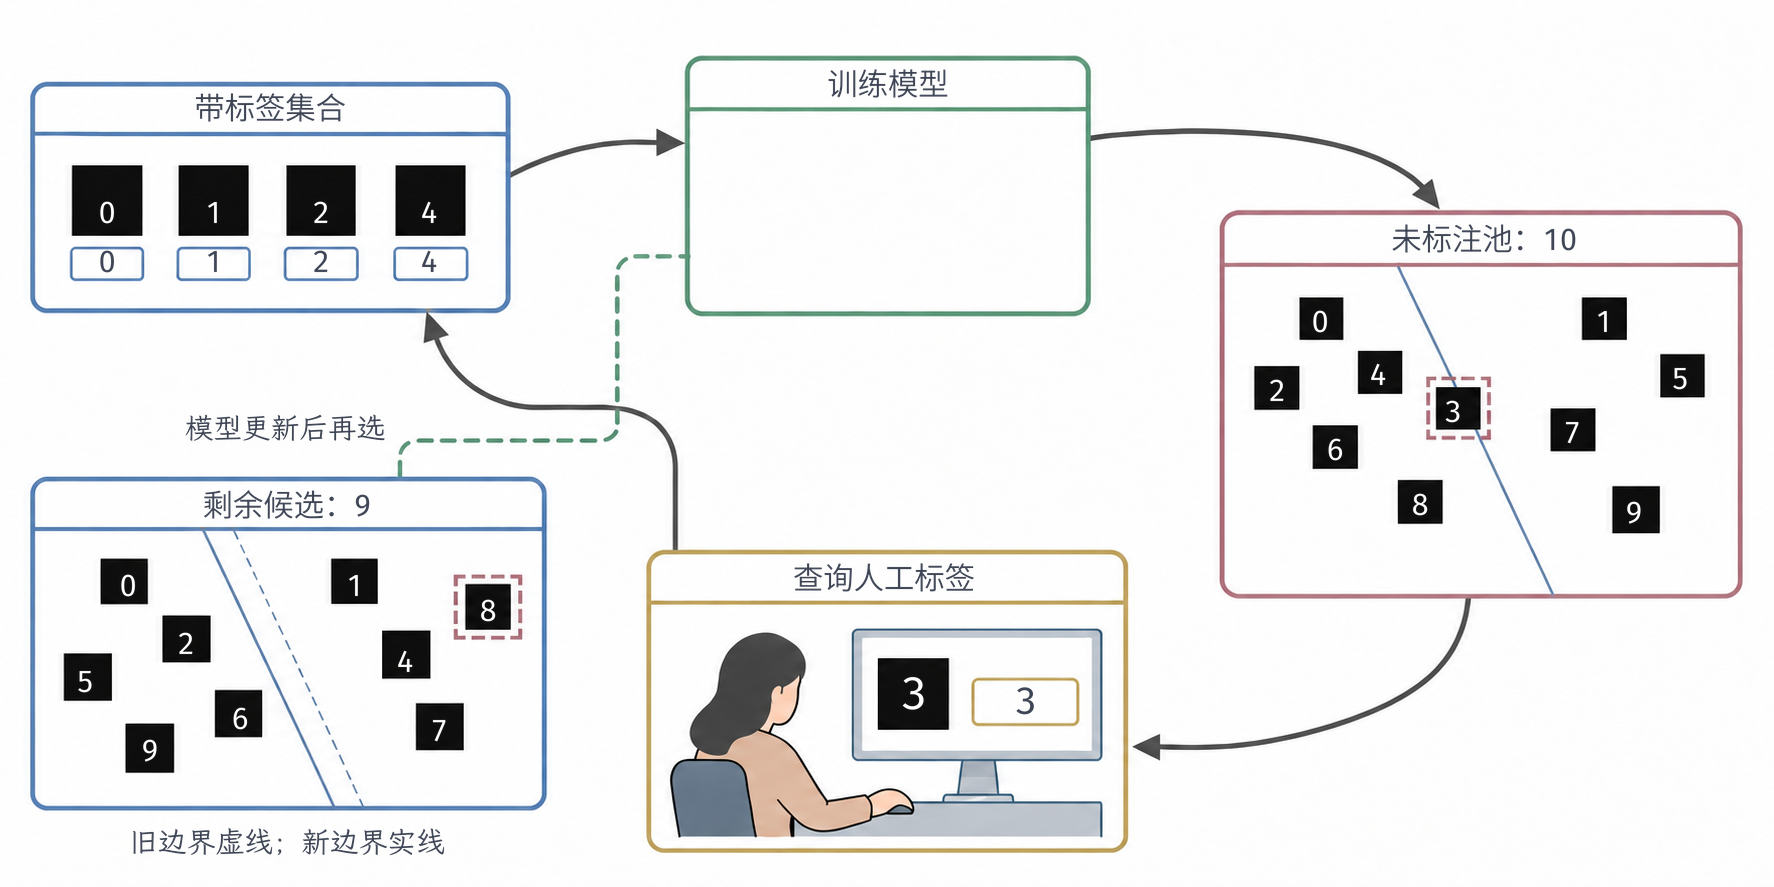
\includegraphics[width=164.600mm]{figures/03-foundations/01-basics/generated/active-learning/figure.png}
  \caption{池式主动学习的教学示意。蓝色直线表示当前模型的决策边界，红色虚线方框标出本轮查询的数字3。标注者返回标签后，样本并入带标签集合，用于重训模型，未标注池由10个候选减为9个。左下方的虚线保留更新前的边界，实线表示更新后的边界；虚线方框标出的数字8是下一轮查询对象。查询预算限制循环。数字字形、二维位置和边界均为教学构造，不表示实测分布或选样收益；数字样本的外观不等同于供模型使用的类别标签。}
  \label{fig:active-learning-loop}
\end{figure*}
\FloatBarrier

不确定性只是选样的一项依据。严重模糊的数字虽让模型犹豫，得到标签却未必能提供可推广规律；不断查询几乎相同的写法，也可能重复信息。我们还要检查覆盖与多样性、回答可靠性，以及各样本的标注成本，才能判断新增标签是否值得。

主动与半监督可以共同用于数字识别：一部分图被选中请求真实标签，其余图通过伪标签或一致性参与训练。查询解决预算怎样分配，半监督解决剩余无标签输入怎样利用，二者承担不同步骤。

主动学习只决定优先询问的样本。答案能否使用，还取决于标注任务和判定规范、直接作答或候选比较等交互方式、标注者能力、复核及预算分配。这些条件同属人工知识获取，需要在查询策略之外说明。

选择与反馈的循环并不自动构成强化学习。本例查询返回图片标签，评价是在给定标注预算下，独立评价集上的数字分类准确率；强化学习以奖励评价行动后果及累计回报。当然，多轮查询也可再建模为序贯决策，并用强化学习寻找策略，但这属于额外实现选择。

\subsection{标签利用方式的比较}
\label{sec:efficient-knowledge-use-comparison}

用同一批少量有标签的花卉照片比较：半监督围绕花卉分类，同时利用标签和未标注输入；自监督先由照片构造目标，学习表示，后续还需类别标签或其他信息规定识别对象。前者利用现有两类数据完成目标任务，后者先解决额外标签缺失时的信号来源。

专家只能提供粗判断，或规则提供有误差标签时，弱监督关注怎样使用和修正这些信号；专家能可靠回答而预算有限时，主动学习关注先询问哪些照片。二者分别限定监督质量与获取过程，节省标注这一共同目的不足以使它们等同。

对比则规定怎样利用样本关系，同源视图或类别标签均可产生匹配目标。因此，它可以与自监督或监督重叠；半监督也可归入广义弱监督。表~\ref{tab:efficient-knowledge-use-comparison}按资源、方式和条件汇总，帮助判断方案适用性，而非要求系统只能选一个名称。

\begin{table*}[htbp]
  \centering
  \small
  \begin{tabularx}{\linewidth}{@{}lXXX@{}}
    \toprule
    \textbf{范式或方法} & \textbf{可以利用的资源} & \textbf{减少标签依赖的方式} & \textbf{需要检查的条件} \\
    \midrule
    半监督学习 & 少量标签与无标签数据 & 让无标签样本也参与目标任务学习 & 数据结构与目标类别是否相符 \\
    自监督学习 & 原始内容及其关系 & 从数据中构造训练目标 & 所学规律是否对实际任务有用 \\
    弱监督学习 & 粗标签、噪声标签或规则 & 接受成本较低的不完善监督 & 标签误差及不同来源的依赖 \\
    对比学习 & 视图、配对关系或类别标签 & 用匹配关系学习可复用表示 & 匹配依据是否可靠；也可使用标签 \\
    主动学习 & 可查询的样本与标注来源 & 优先为有价值的样本获取标签 & 查询收益、样本覆盖与标注成本 \\
    \bottomrule
  \end{tabularx}
  \caption{围绕有限标注比较知识的获取与使用。减少人工任务标签并不等于减少全部训练成本，
  也不保证这些方法在任意数据上都能提高效果。}
  \label{tab:efficient-knowledge-use-comparison}
\end{table*}
\FloatBarrier

同一样本可能得到多来源判断，融合前首先要确认对象、语义及粒度是否对齐，再评估覆盖、偏差和依赖。结果可保留单标签、概率、候选集合或弃权，而不必强行确定答案；一致来源也可能共享错误。标签、关系和约束若无法化为同一语义下的判断，就应保留含义分别参与训练，不能直接投票。

融合后仍需质量处理。我们用独立依据及有代表性的审计样本区分已确认错误、复核线索和信息不足，定位来源或构造环节，再修正、独立验证并记录版本。任务答案可检查正确性，关系与表示目标还要检查构造条件及下游用途。评价标准跟随知识的含义，这些步骤才使候选依据进入可用训练流程。

\section{知识的演进与迁移}
\label{sec:knowledge-evolution-and-transfer-overview}

经验利用还会遇到时间与任务变化。道路识别从白天转到夜间，或从物体类别扩展到距离估计，都会要求检查已有知识能否复用、新旧能力应怎样联系。即使数据与任务未明显改变，也可能需要修正事实或组合分别训练的模型。因此，知识演进不限于分布变化后的重新训练。

\emph{数据变化}可涉及拍摄条件、样本组成及输入与目标的统计关系；从同一分布换一批样本，不代表分布改变。\emph{任务变化}涉及输出、类别范围或评价目标，例如从识别转向距离估计。同一数据可服务不同任务，同一任务也可面对不同分布，需要分开描述。

知识可以承载在样本和外部记忆、表示与关系、预测规则、参数、模块或学习策略中。这些对象以不同方式影响后续学习和预测。参数变化不能直接证明某条事实已正确修改，外部记录存在也不能证明模型会使用；知识载体、能力和事实含义应分别检查。

持续学习关注经验随时间累积，多任务关注跨任务共享，迁移关注来源对目标的帮助，元学习关注怎样改进后续学习。比较时还需说明任务组织、历史访问和评价要求，不能只按数据或任务是否变化分类。下面先讨论新经验到来时怎样保留所需旧能力。

这四种范式为\BookPartRef{part:knowledge-evolution-and-transfer}{第四卷“范式”的“知识的演进与迁移”部分}提供入口。后续会研究复用是否值得、选择哪些知识、怎样更新维护及整合能力，再研究迁移与共享的实际收益。更新保留、共同训练和目标适应可能交叉，也会使用共同的选择、整合与评价方法。

\subsection{持续学习}
\label{sec:continual-learning}

未来经验不能一次收齐：拍摄条件、用户兴趣或类别范围可能陆续变化。\term{持续学习}（continual learning）要求按顺序吸收新经验，同时保留任务仍需要的旧能力。适应与保留必须一起进入评价。

同一参数可能同时支持新旧能力，按新数据更新就可能破坏旧任务。固定旧评价集与指标后，若更新后指标恶化，例如旧类别识别的准确率降低，我们称之为旧能力遗忘；严重时称为\term{灾难性遗忘}（catastrophic forgetting）。所以检查新内容学会以后，还要回到旧内容，而不能只报告最新阶段成绩。

图像类别可以分批到达，每阶段要求识别全部已见类别，且预测时不提示图片来自哪个阶段，这就是\term{类别增量学习}（class-incremental learning）。iCaRL在CIFAR-100和ImageNet上逐步增加类别，并限制保存的旧样本数\scite{rebuffi2017}。图~\ref{fig:continual-learning-timeline}展示评价范围怎样扩大：每次既检查新增类别，也检查旧类别保留。

\begin{figure*}[!tbp]
  \centering
  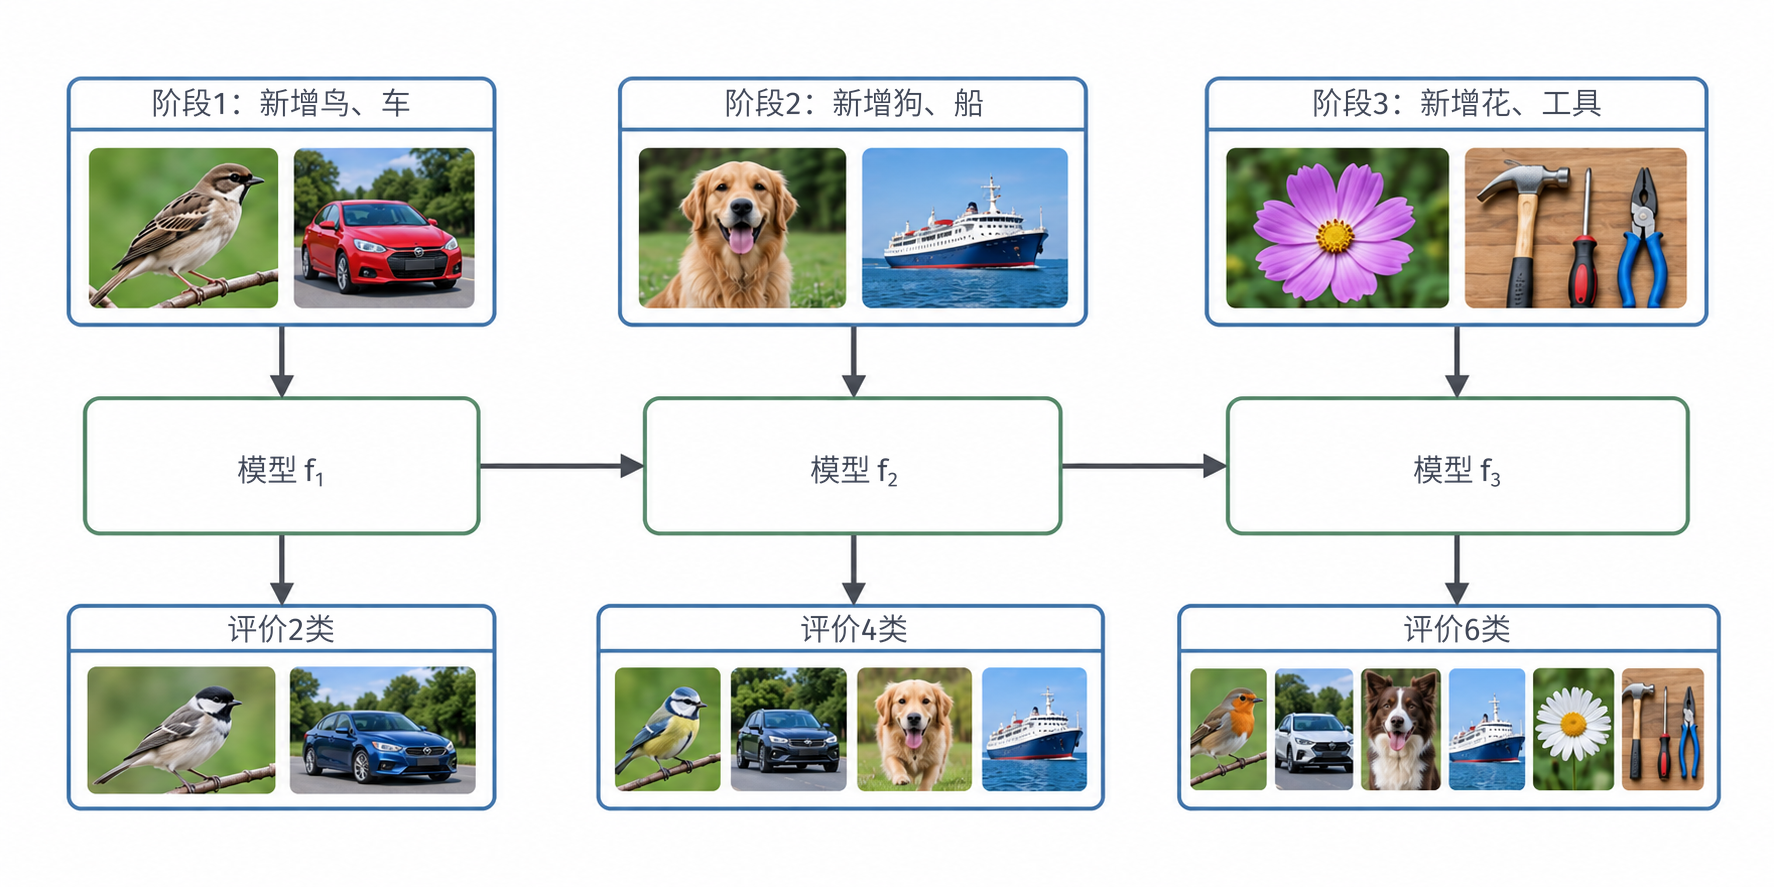
\includegraphics[width=164.600mm]{figures/03-foundations/01-basics/generated/continual-learning/figure.png}
  \caption{持续学习的类别增量过程。不同类别的图像按阶段到来；每个阶段都要学习新增类别，并在截至当前出现过的全部类别上检查能力。横向箭头串接各阶段的模型更新，下方评价范围依次覆盖2、4、6类，预测时不给阶段身份。样本图片为教学构造，模型框不对应精确记忆容量。}
  \label{fig:continual-learning-timeline}
\end{figure*}
\FloatBarrier

这种要求的难度依赖历史访问、任务边界提示和评价时间。全部历史数据可用时，可以重新训练；只能保留少量旧样本时，复习更受限制。持续学习也可处理传感器、兴趣或任务的连续变化，讨论时应先给出这些条件。

预测时若知道当前任务，可以选择相应输出，这构成\term{任务增量学习}（task-incremental learning）。若输出含义保持不变、输入分布陆续改变，且不给任务身份，则是典型\term{领域增量学习}（domain-incremental learning）。它们与类别增量构成常用比较设定\scite{vandeven2019}，分别改变提示、输出范围及分布条件。

白天与夜间都识别同一组交通标志，可以形成领域增量；陆续增加标志种类并在全部已见类别中选择，可以形成类别增量；先告知每次属于哪组识别任务，则更接近任务增量。三者都要按要求保留能力，但结果不能脱离提示和预测范围比较。若目标同时包含白天与夜间，仅夜间改善而白天失效就未满足要求。

更新维护的范围比持续学习更广，还包括修正过时事实、修改指定内容，或消除特定训练记录的影响。对象可以是参数、结构或外部记忆，不必以分布变化为前提。修改后需要分别验证目标内容、相关内容一致性、无关能力保留及后续可学性，并记录版本与恢复方式。

\subsection{多任务学习}
\label{sec:multi-task-learning}

若相关任务的数据能在训练中共同访问，我们可以让它们相互提供信息。街景识别与距离估计都可能需要物体边界，\term{多任务学习}（multi-task learning）通过共享表示或其他知识共同学习各项目标\scite{caruana1997}。一个任务的反馈由此有机会帮助另一个任务；并行运行彼此不联系的模型，并不会产生这一共享机制。

街景中的\term{语义分割}（semantic segmentation）逐像素预测道路、车辆、建筑等类别，\term{深度估计}（depth estimation）估计像素所对应物体的距离。Kendall等人还加入区分物体个体的\term{实例分割}（instance segmentation），研究怎样平衡不同任务的反馈\scite{kendall2018}。

图~\ref{fig:multi-task-learning-process}仅展示语义与深度两项：同图经过共享模块，再分成两路预测，各路与自身标注比较，反馈共同调整共享部分。边界信息可能因此被两项任务复用，各自的预测要求却仍需保留。

任务集合可以固定不变，数据也可以预先收齐，多任务学习并不要求时间变化。各任务既可共享输入而使用不同标注，也可拥有各自数据集。定义所关注的是学习之间的联系，即一个任务的训练能影响另一任务。

多任务与持续学习的区别要看经验组织。训练期间能反复访问各任务数据，即使交替更新，仍可属于共同学习；经验顺序到来且历史无法完整访问时，则更突出持续学习的保留要求。任务数量本身无法区分二者。

\begin{figure*}[!htb]
  \centering
  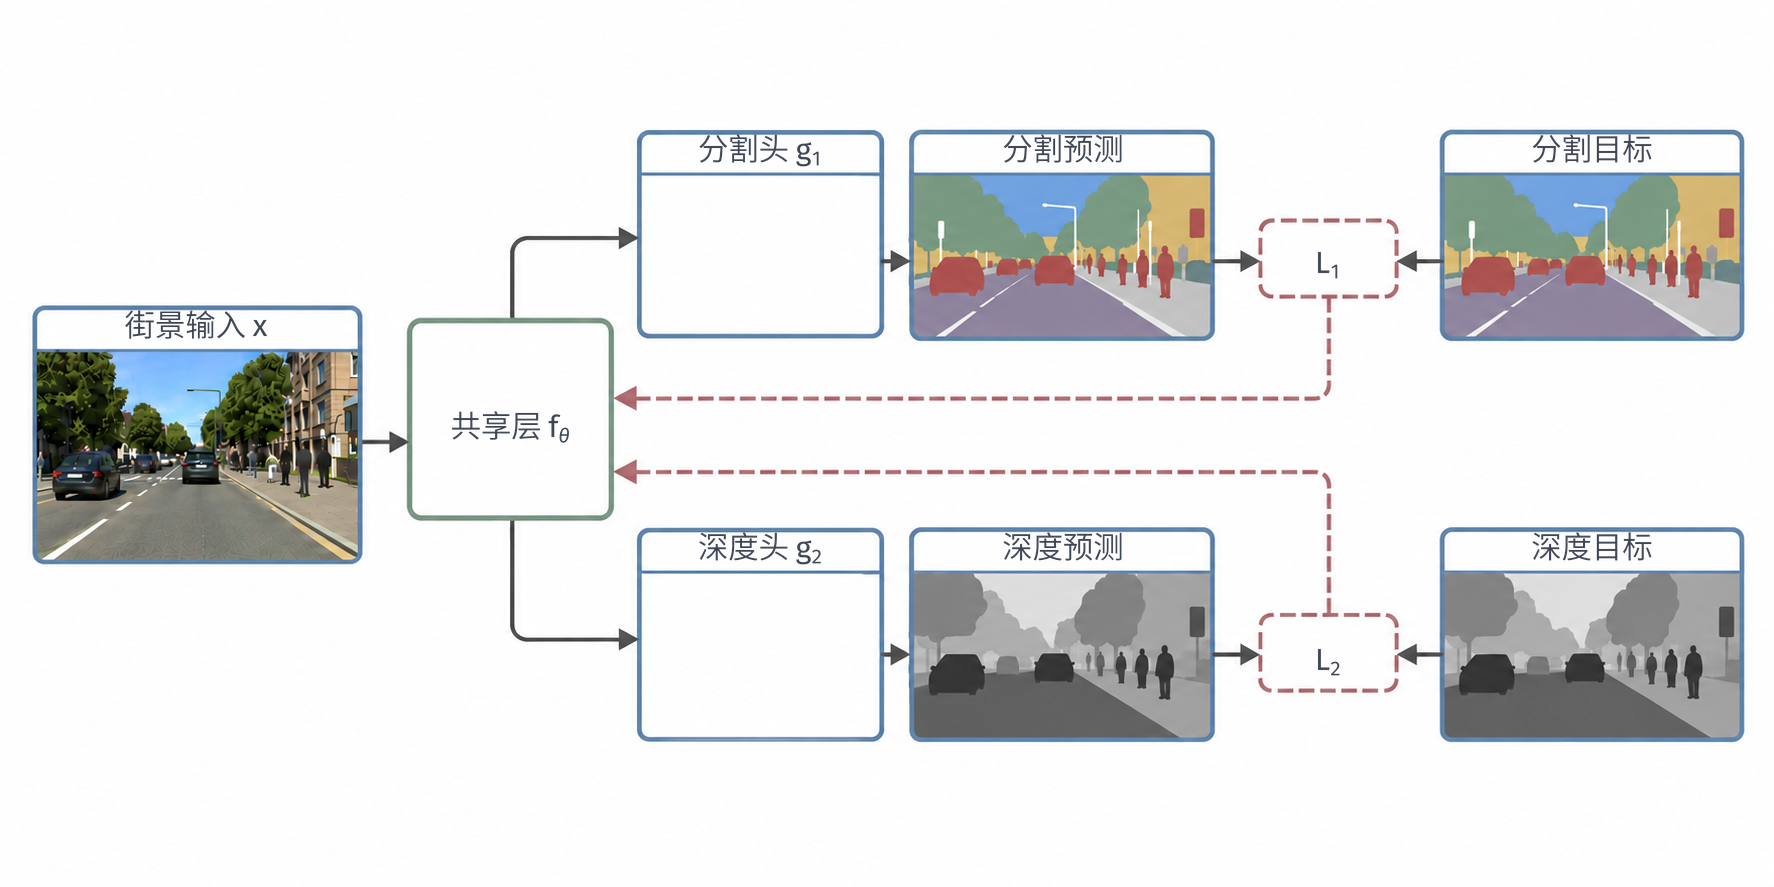
\includegraphics[width=164.600mm]{figures/03-foundations/01-basics/generated/multi-task-learning/figure.png}
  \caption{多任务学习的过程示意。同一街景及不同任务的标注共同影响共享表示，系统分别输出
  语义区域和远近关系；两个结果都是概念示意，不是论文实验的实际输出。}
  \label{fig:multi-task-learning-process}
\end{figure*}
\FloatBarrier

共享可能带来收益，也可能使一个任务的更新损害另一个任务；数据更多或更容易的任务还可能主导表示。我们因而要分别评价各任务，再决定任务分组、共享内容与结构、联合目标，以及样本、更新和计算资源的分配。单个汇总分数不能充分呈现任务干扰。

多任务从共同训练出发；已有模型或模块若先分别学成，再通过预测组合、连接、参数融合或蒸馏协作，则主要属于知识整合。它处理的是已有能力怎样进入新的计算过程，与前述候选标签等训练依据的融合对象不同。

\subsection{迁移学习}
\label{sec:transfer-learning}

已有相关经验还可以帮助一个目标问题。\term{迁移学习}（transfer learning）区分来源与目标，把来源学到的表示、参数等用于目标，减少从头学习的需求。它可帮助标签有限的任务，也可用于加快学习或适应分布变化，但首先要判断哪些来源知识仍对目标有用。

教学中的花卉模型可以先复用ImageNet训练所得图像表示，再用较少花卉标签学习类别。来源提供边缘、纹理及形状等基础，目标标签仍负责规定花卉之间的重要差异。图~\ref{fig:transfer-learning-process}的箭头指明已有表示或参数进入目标学习，目标学习由此从已有图像经验出发。这里的花卉过程是教学情景。

\begin{figure*}[!htb]
  \centering
  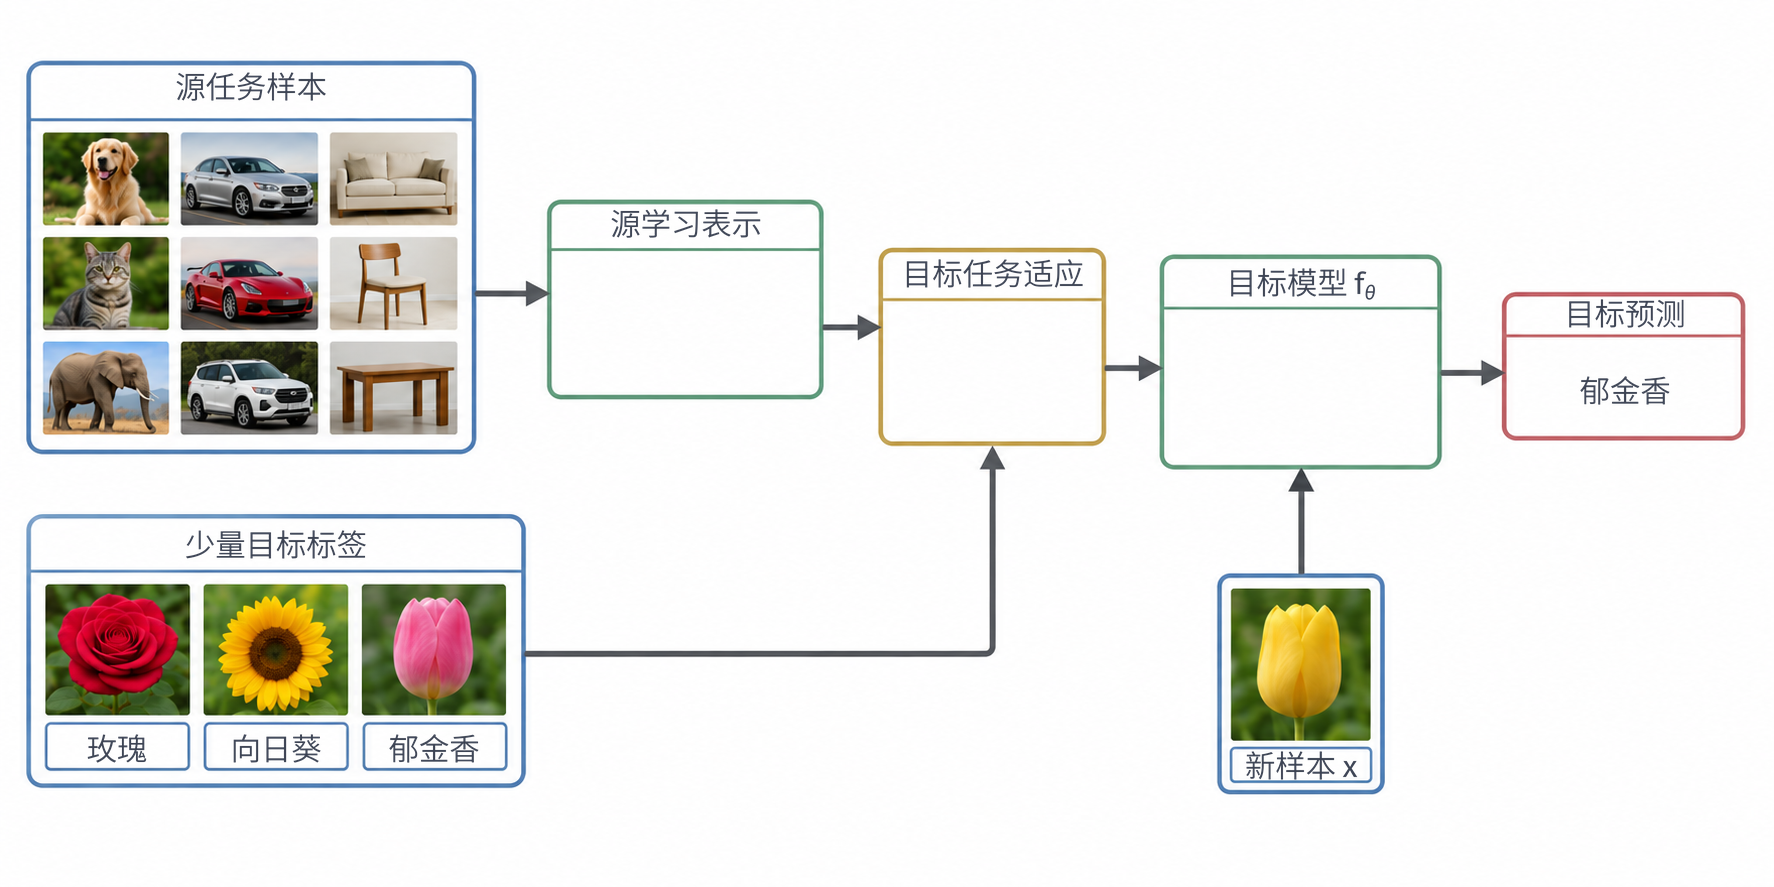
\includegraphics[width=164.600mm]{figures/03-foundations/01-basics/generated/transfer-learning/figure.png}
  \caption{迁移学习的过程示意。通用图像任务形成可复用的表示，目标任务再用少量花卉标签调整
  这些知识，最后识别新的花卉照片；来源知识与目标数据共同决定结果。}
  \label{fig:transfer-learning-process}
\end{figure*}
\FloatBarrier

通用来源不会自动规定花卉分类标准。边缘、颜色和纹理可能共用，但足以区分汽车与动物的特征，未必区分外形近似的两种花。目标标签要使模型进一步关注相应差异。

图像网络早期层常提取边缘、颜色与局部纹理，较后层再形成与训练任务相关的组合。Yosinski等人的研究中，高层特征通常更依赖原任务；在论文比较的任务划分中，来源与目标差异更大时，冻结特征后的目标分类准确率相对于直接在目标上训练的基线下降得更多\scite{yosinski2014}。这一结果须按固定目标评价集及指标理解，不能外推为高层一概不可复用。保留或调整哪些层，仍要针对目标检验。

以来源参数为起点，继续用目标数据调整，称为\term{微调}（fine-tuning）；也可以冻结已有表示，只训练目标输出模块。两者是复用方式，选择依据包括目标数据量、任务差异及允许修改的范围。

信息访问还会限制这些方式。来源可能开放数据、参数、中间表示或模块，也可能只允许查询输出；目标可能提供标签、无标签输入、描述或随后反馈。我们还需记录训练、模型选择及部署各阶段可以使用哪些信息，相同方法名称不能抹去这些条件。

迁移主要补充先前知识，主动学习主要决定获取哪些新标签。花卉系统可先复用图像表示，再查询尚需确认的照片。组合是否有帮助，要同时检查来源相关性及新增标签是否补足目标缺口。

来源到目标不要求数据与任务同时变化。通用分类转到花卉改变类别范围；白天到夜间可以保持类别而改变输入分布。描述迁移时，应逐项说明差异，而非仅称为换了一批数据。

街景中，若深度表示帮助语义分割且最终只关注后者，比较突出迁移；若两项监督共同训练共享表示，并分别评价，则突出多任务。二者可以重叠，迁移也可借共同训练实现，训练先后并非充分判据。持续学习还需按要求保留旧能力，一次迁移则可能只要求目标表现。

在相同目标评价数据和可用目标信息下，若复用来源知识的指标劣于从头学习的基线，例如目标分类准确率更低，称为\term{负迁移}（negative transfer）。判断必须在目标任务上比较，来源规模和来源成绩不能替代证据。复用决策还需比较标签或反馈需求，以及准备、适应、推理与存储成本；效果有益也不保证每种成本口径都更合适。

任务不变而拍摄环境改变时，还要说明目标信息何时可用。本书用\term{域}（domain，也称领域）描述输入空间及其数据分布，\term{源域}（source domain）提供已有知识，\term{目标域}（target domain）是希望模型有效工作的环境。白天、雨天和夜间可呈现不同统计规律；域不由数据集名称唯一决定，同一数据集可含多种环境。

夜间图片可提前收集时，我们可以利用它们适应白天模型。\term{领域自适应}（domain adaptation，也称领域适应）据可用目标数据处理分布差异；有目标标签时属于有监督设定，源有标签而目标只有输入时属于\term{无监督领域自适应}（unsupervised domain adaptation）。域对抗方法尝试保留源分类能力，同时让表示难以区分来源，以辅助迁移\scite{ganin2016}。无监督只限定目标标签，缩小表示差异也不自动保证目标正确。

部署环境尚未确定时，训练和选择阶段无法使用目标数据。\term{领域泛化}（domain generalization）只利用一个或多个源域，要求在未见目标域工作\scite{muandet2013}。例如，以若干城市的白天、雨天图像准备模型，之后直接预测此前未接触的夜间输入。这比同分布新样本评价增加了环境差异，不能假定来源已覆盖未来变化。

这一限制也包括调参、停止时间和模型选择，不能提前借夜间数据作这些决定。可用来源留出域模拟变化；Gulrajani与Lopez-Paz专门研究了选择方式对评价的影响\scite{gulrajani2021}。目标数据在本章标准设定中只用于最终检验。预测当然要读取当前图像，但读取以输出，与利用它更新模型不同。

源域之间稳定的物体形状可能帮助减少背景依赖，但源间稳定并非任意目标稳定，增加源域也不必然改善目标。若未来输入或标签规律任意改变，原经验无法保证成功。领域泛化仍依赖来源与目标可利用的联系，第~\ref{sec:domain-generalization}节将说明学习条件。

部署时可见目标输入，又提供了适应机会。\term{测试时适应}（test-time adaptation）按约定利用测试或部署数据更新参数或统计量，常见设定没有目标标签。Tent用测试输入及预测更新部分参数，以降低预测分布的熵，使类别概率更集中\scite{wang2021tent}，但自信可能伴随错误，更新也可能强化错误。评价要规定输入可见范围、更新时序，以及跨样本是否保留状态。

表~\ref{tab:domain-transfer-settings}以目标信息的可用阶段对照。训练按领域泛化准备、部署继续适应时，系统同时涉及两套条件；报告应说明发生了更新，不能把适应结果计为固定模型的直接泛化。

\begin{table*}[htbp]
  \centering
  \small
  \begin{tabularx}{\linewidth}{@{}lXX@{}}
    \toprule
    \textbf{设定} & \textbf{可用的目标域信息} & \textbf{关键条件} \\
    \midrule
    有监督领域自适应 & 适应时已有目标域带标签样本 & 用目标监督调整模型，另留样本评价 \\
    无监督领域自适应 & 适应时已有目标域无标签输入 & 源域标签与目标域输入共同参与学习 \\
    领域泛化 & 训练及模型选择时均无目标域数据 & 本章标准设定在目标域直接预测，不更新模型 \\
    测试时适应 & 测试或部署时利用目标输入；常见设定无标签 & 按约定更新参数或统计量，并说明数据与时序限制 \\
    \bottomrule
  \end{tabularx}
  \caption{目标域数据的可用性区分领域自适应、领域泛化与测试时适应。前两行区分目标监督条件，
  最后一行强调适应发生的阶段；它们不是完全互斥的分类。}
  \label{tab:domain-transfer-settings}
\end{table*}
\FloatBarrier

目标标签量构成另一项条件。花卉分类每类只给极少带标签例子时，本章称为\term{少样本学习}（few-shot learning）；不提供目标类别的带标签训练例子，而借助先前知识和类别描述等信息时，称为\term{零样本学习}（zero-shot learning）。它们限定目标资源，并不单独规定来源知识怎样获得与迁移。

类别文字要参与识别，模型需先建立图文联系。CLIP共同学习图像与文本表示，让配套图文得分高于同批不匹配组合\scite{radford2021}。这沿用第~\ref{sec:contrastive-learning}节的关系目标，但比较双方变成图像和描述，所得经验也包括视觉内容怎样对应文字。

使用时可把类别写为“a photo of a cat”（一张猫的照片）或“a photo of a dog”（一张狗的照片），比较新图与各描述的匹配得分，再选择最高者。目标分类不再需要新增带标签训练图，因而属于零样本分类。“零”只限定这部分数据，模型仍依赖已有图文经验，也不能据此断言预训练未包含相关概念。

零样本与领域泛化限制不同。前者在此限制目标类别的标签，后者限制目标域数据在训练及选择中的使用。新类别可以出现在已见环境，新环境也可以包含源域已有类别，所以二者需分别判断。

\subsection{元学习}
\label{sec:meta-learning}

若系统反复识别新字符且每次只有几个例子，我们还可以提前练习怎样快速适应。不同小任务提供历史学习经历，适应后的表现再用于改进下一次学习，而不只是复用一个固定表示。

从一组任务的学习经历改进后续学习，称为\term{元学习}（meta-learning）。它可用于少样本适应，也可关注速度或稳健性\scite{hospedales2022}。“学习如何学习”概括的是跨任务经验的作用，实际系统仍需预先规定模型、目标和更新方式。

以反复学习新字符为例，我们可以让模型每次从同一组起始参数出发，用少量示例调整，再用同任务另一批样本检查预测损失。\term{模型无关元学习}（model-agnostic meta-learning, MAML）利用这些适应后的检查损失更新起始参数，以降低之后少样本适应后的预测损失\scite{finn2017}。评价对象由起点自身转向了从起点学习以后的结果。

MAML的Omniglot实验把少数手写字符类别组成一项任务。每项任务从共同参数出发，以少量标签适应，再以同任务另一批样本检查新写法的识别；这些检查损失汇总后更新共同起点，随后继续练习其他任务。这一准备过程称为\term{元训练}（meta-training），反复优化的是后续适应效果。

图~\ref{fig:meta-learning-process}中，任务内检查样本虽未用于该次少量适应，却通过损失参与起点更新，仍属于元训练。最终评价则使用未参加元训练的新任务，字符实验中对应新类别，只考察少量新示例之后的学习效果。两类检查数据不能混用。

\begin{figure*}[!t]
  \centering
  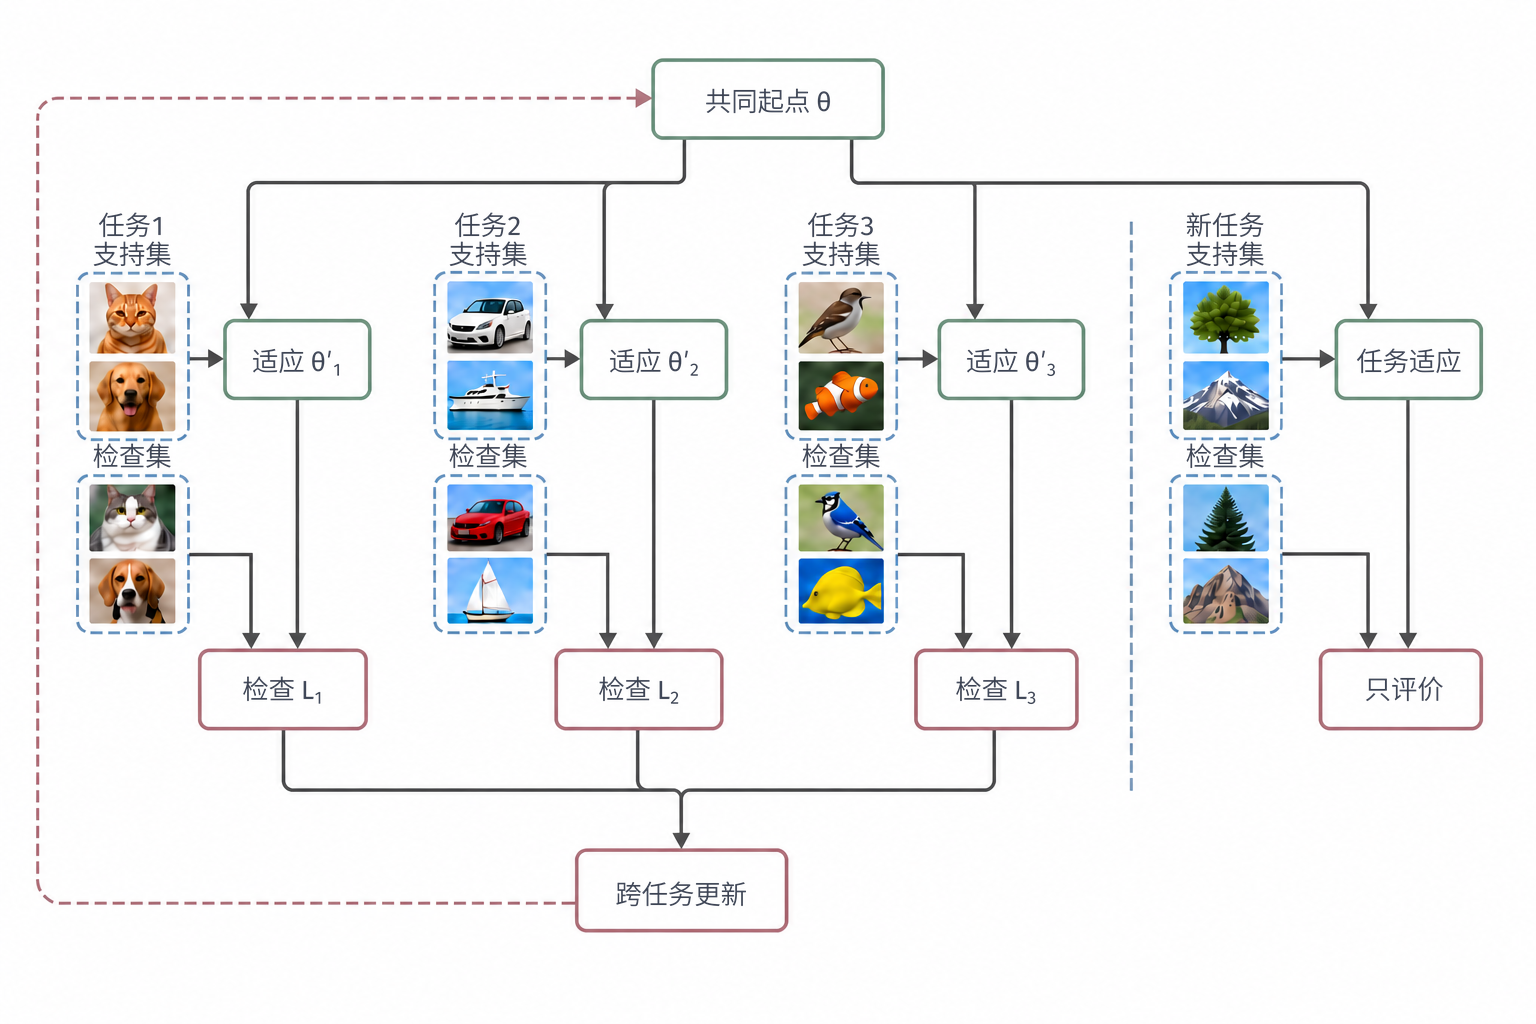
\includegraphics[width=164.600mm]{figures/03-foundations/01-basics/generated/meta-learning/figure.png}
  \caption{任务内适应与跨任务更新。元训练任务从共同起点$\bm\theta$出发，用任务内适应样本得到参数$\bm\theta'_{\tau}$，再汇总另一批检查样本上的损失$L_{\tau}$来更新起点；两批样本都参与元训练。未参加元训练的新任务只用少量适应样本调整参数，最终检查评分不回传共同起点。任务与图像样本为教学构造，不是Omniglot原始样本。}
  \label{fig:meta-learning-process}
\end{figure*}

普通预训练也可迁移参数，差别在准备目标。把旧字符类别合并做监督分类，反馈来自来源识别误差；MAML把数据组织为少样本任务，先适应再检查，反馈来自适应后对该任务新样本的表现。即使两者使用大量旧字符，一个起点为来源识别优化，另一个为少量示例后的学习效果优化。

使用时，两者均可能载入参数再作少量调整，因此要追溯准备阶段才看得出区别。迁移关注来源如何帮助目标，元学习关注历史任务怎样改进学习过程；元学习起点用于新任务也可视为迁移。上述比较仅限定普通监督预训练和MAML，不能把两类范式视为互斥。

少样本只是数据条件，普通迁移等方法同样可以处理\scite{wang2020}。元学习的收益还依赖练习任务与未来任务的联系，差异过大时适应方式可能失效。新任务只给几个例子，也不意味着准备阶段只学过几条数据，它仍可能需要许多历史任务。

例子也可以只进入输入。给语言模型几条评论及其情感标签，再接新评论，让它作答而不更新参数，称为\term{上下文学习}（in-context learning）。GPT-3的少样本实验采用这一方式\scite{brown2020}。因此，使用新示例时要区分输入上下文与参数更新；能利用示例作答本身，也不足以证明曾接受任务适应目标的元训练。

多个训练任务也不足以确定元学习。街景多任务要做好已有分割与深度任务，少样本元学习借历史任务练习适应，再在未见任务上评价。任务承担的用途和最终评价对象，比任务数更能说明设定。

\FloatBarrier
\subsection{数据与任务变化下的比较}
\label{sec:knowledge-evolution-comparison}

表~\ref{tab:knowledge-evolution-comparison}按数据、任务组织及评价汇总四种范式。多任务可以固定任务集合，持续学习可以只面对同任务分布变化，迁移和元学习都可处理新任务；后者还需追溯准备阶段是否改进学习过程。变化的时间、知识服务的对象及能力要求，应与变化本身一起报告。

\begin{table*}[htbp]
  \centering
  \small
  \begin{tabularx}{\linewidth}{@{}lXXX@{}}
    \toprule
    \textbf{范式} & \textbf{数据怎样变化} & \textbf{任务怎样组织} & \textbf{主要评价要求} \\
    \midrule
    持续学习 & 经验顺序到来，分布可能变化；旧数据访问常受限 & 任务可以不变，也可增加类别或依次出现新任务 & 学习新内容，同时保留所需旧能力 \\
    多任务学习 & 各任务可共享输入，也可使用不同数据集；不要求随时间变化 & 一组相关任务共同学习，任务集合可以固定 & 分别检查各任务表现与共享带来的影响 \\
    迁移学习 & 来源与目标的分布可以不同 & 区分来源与目标；目标任务可相同或不同 & 来源知识是否帮助目标任务 \\
    元学习 & 用训练任务积累学习经验，再以新任务数据考察适应 & 跨任务改进学习过程；本节以少样本适应为例 & 在给定适应数据和预算下学得怎样 \\
    \bottomrule
  \end{tabularx}
  \caption{从数据、任务及评价要求比较知识的演进与迁移。各行描述本节的典型设定，
  不是由“变或不变”唯一确定的互斥类别。}
  \label{tab:knowledge-evolution-comparison}
\end{table*}
\FloatBarrier

道路情景可统一比较这些要求。只检查白天知识能否帮助夜间识别，突出迁移；顺序接触环境且保留白天能力，加入持续学习要求；共同训练物体识别和距离估计，体现多任务；用历史场景练习少量示例适应，再在新场景检验，体现这里的元学习。新数据或多个任务可以出现在各设定中，知识组织与评价要求才进一步区分它们。

跨域问题还要按信息时机细分：夜间数据提前参与学习是领域自适应，训练及选择均不可见目标而直接预测是领域泛化，部署后以目标输入更新是测试时适应。除了变化内容，我们必须说明哪些信息在什么时候可用。

这些方式可以沿时间或任务相互连接。多任务表示可成为迁移起点，元学习的适应方式可用于连续任务。组合是否可行，还要检查所需数据当前能否访问，以及评价是否覆盖真正要取得和保留的能力。

评价因而不能只剩当前任务平均分。目标适应要报告效果与代价，持续更新要检查新知识、历史能力及后续可学性，指定修改和能力整合还需检查修改范围、来源能力及组合结果。人工、计算、存储和维护成本也应分别呈现，无换算依据时不宜混为一个数。

\section{其他范式}
\label{sec:other-learning-settings}

反馈及目标确定以后，经验还可能逐条到来，或分散于不同设备。前者限制预测和更新时序，后者限制数据存放及协作方式。本节以在线和联邦学习说明这些发生条件，它们可以附加到前述范式上。

第四卷因此不为两者各设并列部分：在线时序进入交互或更新问题，联邦组织进入相应协作设定，工程实现继续由系统卷展开。

\subsection{在线学习}
\label{sec:online-learning}

经验持续到来时，学习者可以先用当前模型预测或决策，取得后续反馈再更新，然后处理新输入，这一时序称为\term{在线学习}（online learning）。相对的\term{批量学习}（batch learning）先对给定一批数据训练，再使用所得模型。区别在于经验进入更新的安排。

广告系统先根据内容与展示场景预测点击，之后观察点击结果并更新，提供了实际案例\scite{mcmahan2013}。结果给出监督目标，在线规定其到达与使用时序；反馈可延迟，更新也可按小批次进行。联网或实时响应本身并不构成在线学习，若新反馈从不改变模型，系统只是持续预测。

图~\ref{fig:online-feedback-order}对照反馈更新与固定参数预测。评价应保存尚未获得反馈时的输出，随后更新才作用于后续输入。

\begin{figure*}[!tbp]
  \centering
  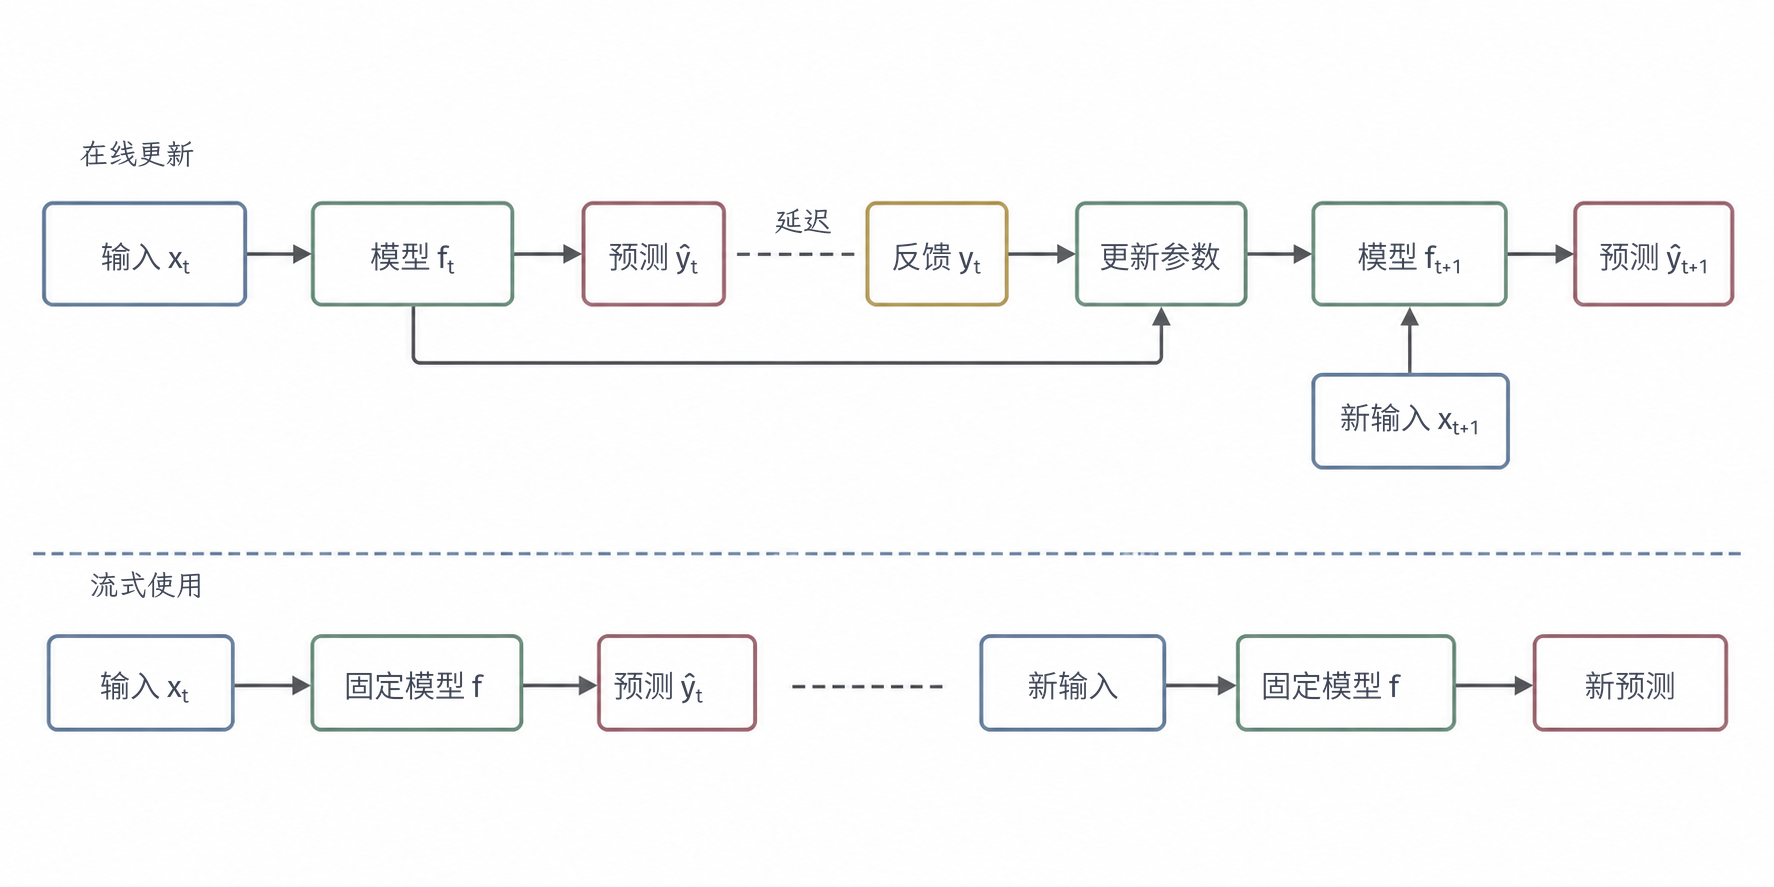
\includegraphics[width=164.600mm]{figures/03-foundations/01-basics/generated/online-feedback-order/figure.png}
  \caption{在线学习先用当前模型预测并保存此时尚未看到答案的结果，反馈可以延迟或按小批次到达，随后更新只作用于后续输入。下方对照只用固定参数持续响应的实时预测；请求持续到来本身不构成在线学习。}
  \label{fig:online-feedback-order}
\end{figure*}

在线与持续学习可以重叠，但各自限定不同条件。同分布样本也可依次预测和更新，在线并不要求任务变化或专门保留旧任务；持续学习关注长期适应与保留，也可按批次阶段更新。若系统逐次学习反馈且检验旧能力，就同时满足两种描述。

随时间改变的数据统计规律称为\term{分布漂移}（distribution drift）。其中\term{概念漂移}（concept drift）在本书专指给定输入后的目标规律变化，例如同样广告与用户特征不再产生原有点击倾向；常见用户或广告比例改变则属于输入或协变量漂移。两者可并存，却有不同识别和调整条件，可能需要检测或改变历史经验权重\scite{bifet2007}。在线只提供利用新反馈的时序，不能保证克服漂移，还受反馈延迟和样本不足限制。第~\ref{sec:distribution-shift}节将形式化区分变化部分。

在线评价必须遵循真实信息顺序。先保存未见答案时的预测，反馈到达后再更新；若重算已经用于更新的样本，就不能还原当时表现。反馈延迟、数据保留量及更新预算也要报告，它们规定模型何时、凭多少经验改变。

\subsection{联邦学习}
\label{sec:federated-learning}

手机键盘需要多样用词经验，但单台设备只有部分记录，原文本又不便集中。这里的困难是共同利用分散经验，而未必是总体样本数不足。我们需要一种保留本地数据的协作安排。

\term{联邦学习}（federated learning）让设备或机构保留本地数据，通过交换模型相关信息共同训练。手机键盘研究在设备端学习下一词，再汇总本地结果改善共享预测\scite{hard2018}。下一词目标由原文本构造，属于自监督来源；联邦则规定各地经验如何协作，二者限定不同方面。

中心协调的一轮先下发共享模型，各设备从它出发用本地数据训练，再上传所得参数。\term{联邦平均}（federated averaging, FedAvg）以样本量加权汇总\scite{mcmahan2017}。令本轮参与集合为$I_t$，第$i$方数据为$D_i$，$n_i=|D_i|$，并要求参与方的总样本量大于零。样本量及加权参数写为
\begin{equation}
  n=\sum_{i\in I_t}n_i,\qquad
  \bm\theta^{(t+1)}
  =\sum_{i\in I_t}\frac{n_i}{n}\bm\theta_i^{(t+1)}.
  \label{eq:fedavg-overview}
\end{equation}
$\bm\theta_i^{(t+1)}$表示从$\bm\theta^{(t)}$出发完成本地训练的参数，所以样本多的参与方获得更大权重。公式使用训练后参数，更新也可另表示为改变量；改用其他权重则需说明。图~\ref{fig:federated-learning-process}展示下发、本地学习和汇总的循环。

\begin{figure*}[t]
  \centering
  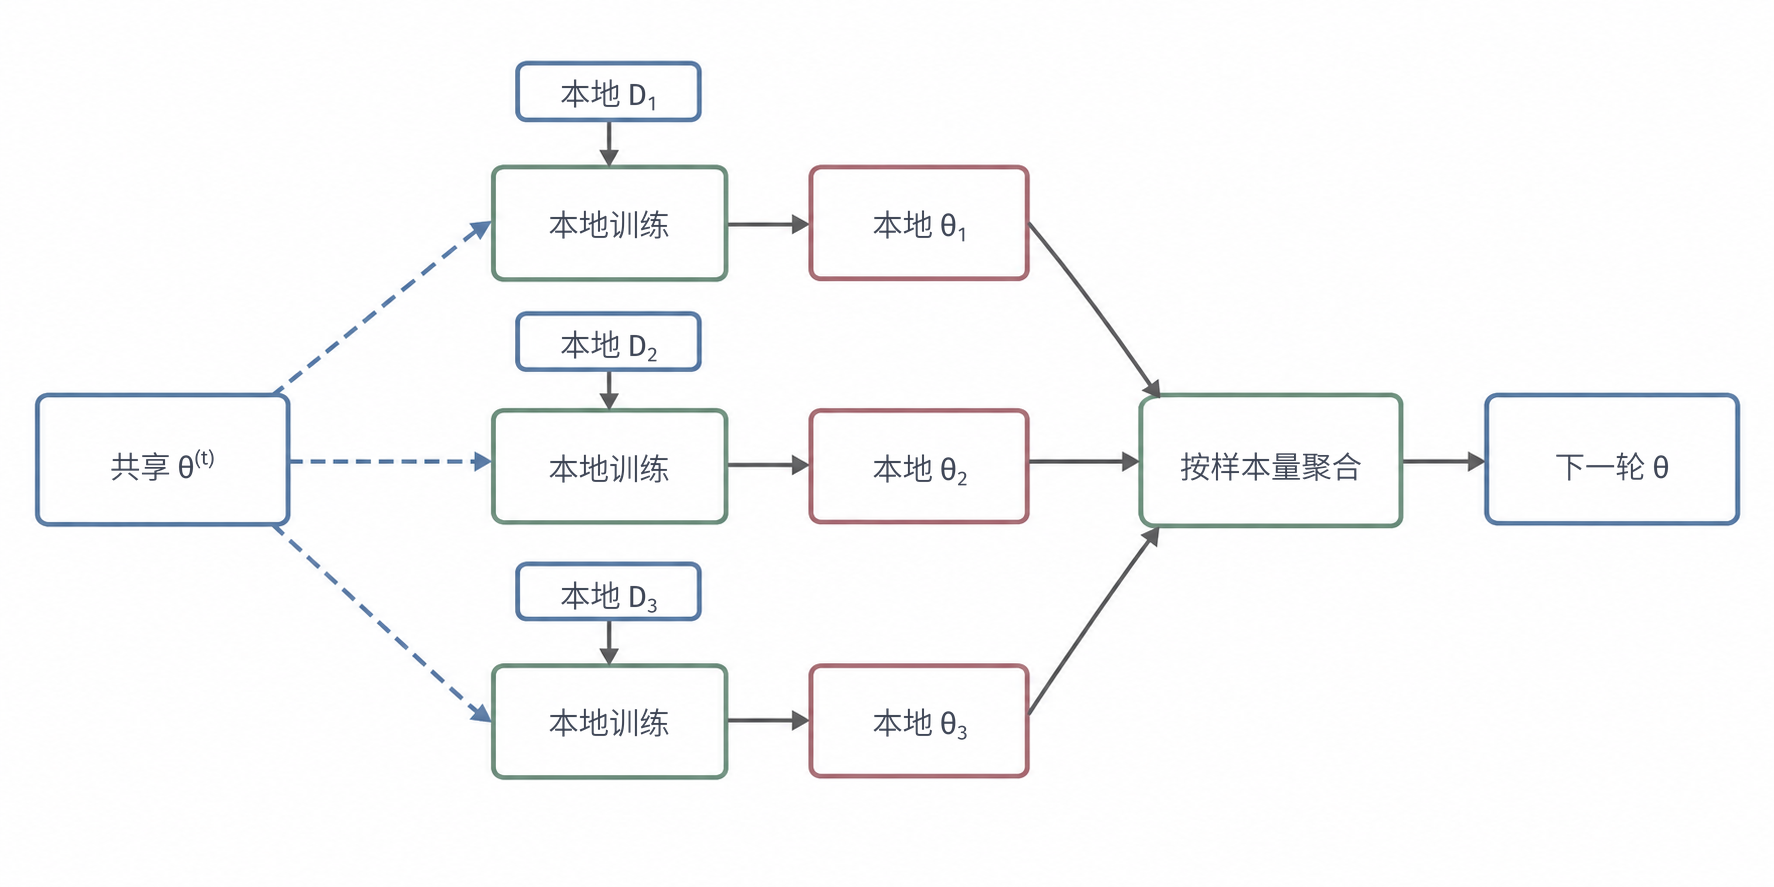
\includegraphics[width=164.600mm]{figures/03-foundations/01-basics/generated/federated-learning/figure.png}
  \caption{中心协调式联邦学习的一轮通信。协调方向三个示意参与方下发同一组共享参数$\bm\theta^{(t)}$；各方使用自己的本地记录集$D_i$训练，得到本地参数$\bm\theta_i^{(t+1)}$并上传。协调方按正文所述的样本量权重形成下一版本$\bm\theta^{(t+1)}$，下一轮再统一下发。参与方数量为教学示意；原始记录留在本地，但模型更新仍可能泄露信息，联邦组织方式本身不提供隐私保证。}
  \label{fig:federated-learning-process}
\end{figure*}
\FloatBarrier

协作会遇到数据量、算力和在线状态的差异，也要承担反复下发及上传的通信成本。原记录留在本地，更新仍可能泄露信息，隐私还需额外机制，例如限制单设备更新的可见性。聚合、通信及部署由\BookPartRef{part:systems}{第六卷“系统”的“机器学习系统”部分}展开，隐私机制由第\ref{part:trustworthy-ml}部分讨论。

共享模型也不一定适合每个用户。设备可迁移共享知识以适应本地，也可用多任务组织保留参与方差异；习惯沿时间改变时，还需检查持续学习。分散协作、个体适应与旧能力保留因而可能共同构成一项系统任务。

\section{范式的组合}
\label{sec:combining-learning-paradigms}

范式分别限定反馈、标签利用、复用及时序环境，同一系统可以跨阶段组合，也可以在同阶段使用多种信号。说明组合时，应逐步追踪数据、目标和反馈，交代哪些知识传给下一步，才看得出每种设定承担的职责。

自监督文本预训练之后用任务标签监督学习，形成分阶段组合：前者积累表示，后者调整到分类、问答等用途。半监督则在同一目标任务中共同使用标签与未标注输入，还可另加自监督目标。二者虽都有多种信号，却不能省略阶段和任务组织的差别。

2016年AlphaGo先以专家棋谱的局面和落子训练策略网络，再用自我对弈的胜负继续改进\scite{silver2016}。传到后一阶段的是初始策略，反馈从专家动作变成对局结果。图~\ref{fig:paradigm-combination-alphago}只展示这条主线，完整系统还有价值网络与搜索等组件。自我对弈使用奖励，属于强化学习，不能因“自我”二字将其归为自监督。

\begin{figure*}[!tbp]
  \centering
  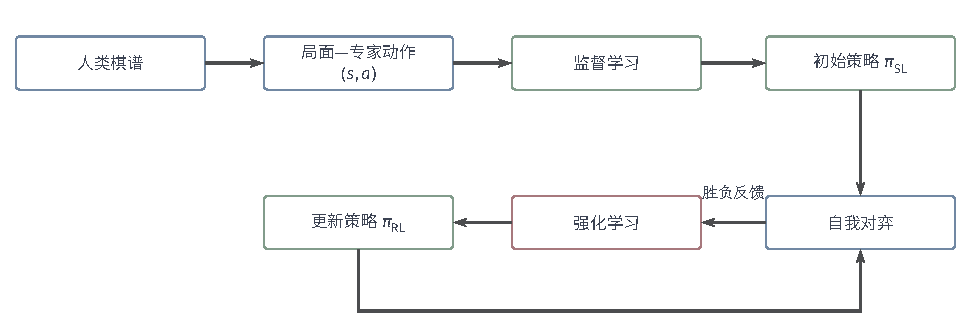
\includegraphics[width=164.600mm]{figures/03-foundations/01-basics/tikz/alphago-learning-path/figure.pdf}
  \caption{AlphaGo学习主线的简化示意。人类棋谱为监督学习阶段提供局面与专家落子；得到初始策略后，
  自我对弈产生新棋局与胜负反馈，用于强化学习阶段。完整系统还包含价值网络与搜索等组件。}
  \label{fig:paradigm-combination-alphago}
\end{figure*}
\FloatBarrier

难以逐步打分时，人可能仍能比较两段行为。\term{偏好学习}（preference learning）利用这种相对判断；与强化学习组合时，可先请人选出更符合要求的片段，据此训练评价模型，再用所得奖励训练智能体。相关研究用于Atari和模拟机器人\scite{christiano2017}。这里人提供行为好坏比较，未直接给每步动作；评价模型转成奖励，策略再依据奖励学习。

在假设的多机构花卉系统中，各机构保留照片，以联邦方式协作；本地无标签照片产生不同视图，通过自监督对比目标学习表示。联邦规定协作，自监督规定匹配来源，对比规定目标构造。这些描述可以共同成立，却不能互相替代。

系统还可主动查询部分专家标签，再结合剩余未标注照片作半监督训练；通用表示可迁移，新物种陆续加入时可检查持续学习。该情景用于解释组合，实际方案按需求选用环节即可。标签选择不替代目标学习，协作也不会自动消除来源差异、错误或遗忘。

\section{本章小结}
\label{sec:machine-learning-paradigms-summary}

本章从经验和反馈建立范式，而非仅按模型名称分类。任务规定目标，模型表达候选规律，范式组织学习依据。监督以输入和目标配对，无监督发现结构或分布，强化学习利用行动奖励改善决策。先追溯系统实际得到什么，再确定训练与评价的条件，才能说明学习怎样发生。

标签不足时，可以让未标注输入参与任务、由数据构造新目标、接受并处理较弱监督，或主动获取关键答案；对比学习则规定如何利用样本关系。这些方式都依赖信号可靠且符合任务，减少人工标签不能自动保证能力。人工、规则、模型与数据提供的候选知识，还需对齐、融合、评估和修正。

经验演进后，持续学习强调顺序适应与保留，多任务强调共同共享，迁移强调来源对目标的帮助，元学习强调历史经历对后续学习的改进。在线与联邦分别限定更新时序和协作，目标信息的可用阶段又区分领域适应、泛化与测试时适应。组合时，应说明数据、反馈、任务关系与信息权限，再评价实际需获得和保留的能力。已有表示、参数、模块、记忆及学习策略怎样复用、更新或整合，也须分别检查效果和样本、计算、存储及维护代价，在明确预算下取舍。

\paragraph{延伸阅读}

继续学习交互决策可读Sutton与Barto教材，标签质量及任务适应可分别参阅弱监督与元学习综述，联邦平均原始论文提供分散协作的具体入口\scite{sutton2018,zhou2018,hospedales2022,mcmahan2017}。结合第~\ref{chap:machine-learning-models}章，我们已有表示规律和利用经验的基本框架。第\ref{part:learning-theory}部分将在给定经验、损失及比较标准下研究有限样本能否学到所需结果，第\ref{part:trustworthy-ml}部分检查其进入流程后的可靠性、鲁棒、公平、隐私、安全与处置要求。\BookPartRef{part:reinforcement-learning}{第四卷“范式”的“强化学习”部分}、\BookPartRef{part:efficient-knowledge-use}{“知识的获取”部分}及\BookPartRef{part:knowledge-evolution-and-transfer}{“知识的演进与迁移”部分}再分别展开交互决策、训练依据和已有知识的利用，协作部署继续连接系统卷。
